 \documentclass{IEEEtran}
\usepackage{cite}
\usepackage{amsmath,amssymb,amsfonts}
\usepackage{algorithmic}
\usepackage{graphicx}
\usepackage{textcomp}
\usepackage[utf8]{inputenc}
\usepackage{booktabs}
\usepackage{multirow}
\usepackage{tabularx}
\usepackage{color}
\def\BibTeX{{\rm B\kern-.05em{\sc i\kern-.025em b}\kern-.08em
    T\kern-.1667em\lower.7ex\hbox{E}\kern-.125emX}}

%%Isabel's comments
\newcommand\fia[1]{{\color{red}\footnote{\color{red}from Isabel: #1}}} %change to 
\newcommand\dia[1]{{\color{blue}\footnote{\color{blue}from Felipe: #1}}}
%\newcommand\fia[1]{} %to remove all comments
\newcommand\mc[1]{{\color{green}\footnote{\color{green}from Marwa: #1}}}
\newcommand\juli[1]{{\color{magenta}\footnote{\color{magenta}from Juli: #1}}}

\newcommand\mia[1]{{\color{red}#1}}%change to 
%\newcommand\fia[1]{} %to remove all modifications, or to 
%\newcommand\mia[1]{{#1}}% to accept them

\newcommand\delia[1]{{\tiny{\color{red}#1}}} %change to 
%\newcommand\fia[1]{#1} %to discard all modifications, or to 
%\newcommand\mia[1]{{}} %to accept all changes

\begin{document}
\title{The Controller Placement Problem in Software Defined Networking: A Systematic Review}
\author{First A. Author, \IEEEmembership{Fellow, IEEE}, Second B. Author, and Third C. Author, Jr., \IEEEmembership{Member, IEEE}
\thanks{This paragraph of the first footnote will contain the date on 
which you submitted your paper for review. It will also contain support 
information, including sponsor and financial support acknowledgment. For 
example, ``This work was supported in part by the U.S. Department of 
Commerce under Grant BS123456.'' }
\thanks{The next few paragraphs should contain 
the authors' current affiliations, including current address and e-mail. For 
example, F. A. Author is with the National Institute of Standards and 
Technology, Boulder, CO 80305 USA (e-mail: author@boulder.nist.gov). }
\thanks{S. B. Author, Jr., was with Rice University, Houston, TX 77005 USA. He is 
now with the Department of Physics, Colorado State University, Fort Collins, 
CO 80523 USA (e-mail: author@lamar.colostate.edu).}
\thanks{T. C. Author is with 
the Electrical Engineering Department, University of Colorado, Boulder, CO 
80309 USA, on leave from the National Research Institute for Metals, 
Tsukuba, Japan (e-mail: author@nrim.go.jp).}}

\maketitle


%\begin{document}

%\maketitle


\begin{abstract}
Software Defined Networking (SDN) is a promising paradigm that enables flexible management of networks by decoupling the control plane from the data plane. It allows controlling the network through one or multiple controllers centrally. However, deciding the number of controllers to deploy in a network and their locations is a particular task which can directly affect the overall network performance. This problem is widely investigated in the literature, and the existing evaluations are varied and diversified. This work aims to synthesize the existing solutions to outline the state-of-the-art and identify limitations and future scope in the hope of providing clarity to the problem. Based on a conceptual evaluation model, the Systematic Literature Review (SLR) method is employed to collect relevant works investigating the Controller Placement Problem (CPP). This review systematically evaluates research on CPP based on questions formulated for this purpose. It classifies the existing solutions based on different criteria, discusses the limitations of the proposed schemes, and points out the non-investigated scenarios related to the studied problem. This paper, which is, to the best of our knowledge, the first attempt of an SLR on CPP, can be a stable basis for potential researchers in this area to address the problems mentioned above.
\end{abstract}
\begin{IEEEkeywords}
Software defined networking, controller placement, systematic review
%Enter key words or phrases in alphabetical order, separated by commas. For a list of suggested keywords, send a blank e-mail to keywords@ieee.org or visit \underline {http://www.ieee.org/organizations/pubs/ani\_prod/keywrd98.txt}
\end{IEEEkeywords}



%\begin{itemize}
%    \item Traditional networks
%    \item Scalability, introduction of SDN
%    \item The CPP, NP-hard, to place the optimum number of controllers on the best locations
%    \item Basic problem introduced by Heller
%    \item Multi-controllers issues
%    \item Motivation
%    \item Paper's outline
%\end{itemize}

\section{Introduction}
In traditional networks, the control plane and the data plane are bundled inside the networking devices. The need to configure each individual network device makes traditional networks complex and hard to manage. Therefore, the idea of a programmable network was born out and updated until the appearance of SDN. SDN is changing the way networks are designed and managed. It separates the control and data plane and it promotes logical centralization of network control and introduces the ability to program the network \cite{OmSe16}. 

Initially, SDN control plane proposals focused on a centralized solution, based on a single control entity which has a global view of the network. The performance of these networks can be greatly improved by carefully choosing the placement of the controller. This was the main work of Heller \emph{et al.} in \cite{HeSh12} which formalized the CPP, although there had been at least a previous consideration of the controller location \cite{ZhBe11}. As presented by these works, the centralized solution presents scalability limitations as the size and dynamics of the network increase. To overcome these limitations, other approaches based on multiple controllers were proposed in order to ensure flexible, evolutionary and convergent network. An important parameter to consider while doing so is the propagation delay between the controllers and the network devices, especially in the context of large topologies. Many other problems can evolve, such as reliability, resilience, cost, etc.  These facts encourage researchers to investigate the multiple CPP, with the aim to optimize the network performance.  Various works have arisen to address the CPP with different optimization goals, such as latency, reliability, load balancing, power consumption, cost, and others. Moreover, in a network it is very common to require more than one performance objective, so multi-criteria proposals are a relatively large group of work in the literature.

Regardless the objective optimized by the CPP, each proposal addresses the problem proposing exact, heuristic or both optimization techniques. Most approaches for exact optimization algorithms in CPP include integer programming, game theory/bargaining games, mixed integer linear programming, and others. On the other hand, for heuristic algorithms, there are works using particle swarm optimization, simulated annealing, genetic algorithms, and others. Additionally, the selection of the metrics is also diverse. Even though there are similarities, several researchers propose particular metrics and evaluation parameters for the presented technique. The lack of unified criteria results in a wide variety of possible research directions that do not provide a clear path to solve CPP. 
 
%\mia{A} typical result is that a selected location is better than a randomly selected one.

%In a traditional network, the control plane is integrated with the data plane, it is sought to decouple the planes of data and control forwarding in SDN networks. The performance of the network can be improved by choosing carefully the location of controllers. This proposes a flexible, evolutionary and convergent network. Those who do not agree, say there will be problems about decision latency, availability, and scalability. For this reason, two questions are asked: how many controllers are necessary and where should they be placed? (how to assign switches to controllers too)

%%The CPP was firstly introduced by Heller et al. in \cite{HeSh12}. The authors only focus on the propagation delay and present an exhaustive search to determine the optimal controller placement within the network topology. By analyzing the performance of controllers in different network topologies, the authors conclude that one controller is often enough to keep the latency at a reasonable rate. Many later works only target the latency as an optimization objective while placing the controller. TODO_M

%%However, even though a single controller could be enough for topologies \cite{HeSh12} from latency point-of-view, more controllers might be necessary to meet resilience requirements. Moreover, a single point of failure obtained with an SDN network with only one controller is not desirable. TODO_M

To define common elements and establish a road-map to solve the CPP for different scenarios, it is necessary for researchers to understand the current landscape of the proposals.

There have been previous attempts to provide an overall view of the CPP \cite{SoXi17}, \cite{KuSr18},\cite{HuGu17},\cite{TaAl17}. However, they lack a systematic approach for the review, which could cause to left out essential aspects of the problem.

The goal of clarifying state-of-the-art techniques requires to address the aforementioned said diversity in experimental forms and evaluation criteria for CPP, with a methodical process. Systematic Literature Review  (SLR) \cite{BuBr06} is an accepted approach to investigate specific research questions and objectively review the literature. In this paper, we adopt such method aiming to identify research gaps and provide a solid foundation for future CPP research activities.

This paper presents a review of most relevant papers discussing the CPP based on the SLR methodology. It answers several research questions in order to classify the reviewed works and to clarify the different research directions related to the studied topic. Based on the discussed questions, the papers are arranged either based on the optimization objectives of the mathematical problem, or depending on the nature of the proposed solutions, and the experimental process established to evaluate the methods. The research questions and papers' classification are detailed in upcoming sections.

%This paper presents the SLR methodology used to review the CPP XXXXX

The rest of the paper is organized as follows. Section \ref{sec:SLR} presents details about the SLR performed in this study. 

\section{Systematic Literature Review}
\label{sec:SLR}

A systematic review essentially provides an exhaustive summary of relevant literature for a specific field of study. It collects and critically analyses research studies according to a structured methodology to answer predefined research questions. As a result, a systematic review offers a firm foundation to a research topic and opens new approaches for further progresses in the concerning field of study. Based on the guidelines for performing SLR \cite{KiCh07}, we establish our review to identify, interpret and analyze all available evidence related to the controller placement problem in software defined networks.


\subsection{Research questions}
Corresponding to the main objective of this SLR that is to examine the proposed methods to solve the CPP and to show the different challenges and opportunities that are posed based on this problem, six research questions were formulated to guide the evaluation process step by step, as listed in Table \ref{tab:QRs}.

\begin{table}[!h]
    \centering
    \begin{tabular}{l p{3.2cm} p{3.6cm} }
  \hline
  ID & Research Question & Main Motivation \\
  \hline
  RQ1 & What are the purposes of solving the CPP? & To identify the optimization objectives of investigating CPP. \\
  RQ2 & What are methods used to solve the CPP? & To identify the optimization methods used to solve the CPP. \\
  RQ3 & How are the methods evaluated? & To describe the experimental process established to evaluate the methods. \\%ie simulation, emulation, real implementation
  RQ4 & What is the experimental setup to evaluate the test scenarios? & To explore the different scenarios used to test the proposed methods. \\ %ie diversity and scale of the used topologies
  RQ5 & What are the case study assumptions? & To determine the specific context considerations and restrictions of the proposed solution.\fia{I don't really understand, isn't it rather To determine the applicability of the solution? for instance?} \dia{I think in this question, we should talk about the constraints defined in the proposed solutions.} \\
  RQ6 & What are the metrics evaluated by the proposed work? & To point out the metrics used to compare different evaluations.\fia{If Im not mistaken, we had considered two different things, one is criteria as the objective function, and the other is other performance criteria used to evaluate the technique. This question refers to what exactly?} \dia{This question refers to the evaluated metrics (column D in the excel file )} \\
  \hline
\end{tabular}
    \caption{Research questions}
    \label{tab:QRs}
\end{table}\fia{the objective of the optimization problem is covered by which one of the questions?}\dia{By RQ1}

\subsection{Research scope and strategy process}
This study focuses on the solutions proposed by the literature to solve the CCP in a WAN SDN, to optimize three factors: 1)  minimum number of controllers required, 2) location of the controller(s) in the network nodes, and 3) how many networking devices (nodes) should be assigned to a given controller.\dia{from where these statements come from?} \mc{from \cite{SiSr18}}

To define a precise publication span, we consider that although the term "controller placement problem" started to gain popularity in 2012 with Heller et al. \cite{HeSh12}, Zhang et al. were the first authors to discuss the controller location in a network in 2011 \cite{ZhBe11}. So, the publication time span of our survey covers the papers from 2011 until the time of conducting the study. 

The \delia{most suitable search terms} \mia{keywords} we used to conduct our study were: "controller placement", "SDN", "WAN", "facility location", "control management", "switch assignment", along with the metrics optimized in the studied problem such as: "reliability", "resilience", "QoS", etc. These keywords allowed us to form several search strings such as: ("controller placement" OR "control plane management" OR "switch assignment" OR  "resilience" OR "reliability" ) AND ("software-defined networking" OR "SDN" OR  "WAN"). 

The inclusion and exclusion criteria can be presented as \mia{follows}\fia{and the inclusion?} \mc{What's the problem here?}:


\subsubsection{Inclusion criteria}
\begin{itemize}
    \item Publications that formulates the CPP and present a solution \dia{Why this paper? I don't see the relationship with the statement.} \mc{You're right I think we don't have to give examples here since all the studied papers are included} \juli{removed}.
    \item Publications that describe the algorithms used to solve the CPP.
    \item Publications that present the results of experiments of the methods used to solve the CPP.
\end{itemize}

\subsubsection{Exclusion criteria}
\begin{itemize}
    \item Publications that describe only theoretical discussions or solve only part of the problem \cite{RaMa18, TaBj18, AdAd18, WaLi2017, HoHa14, HoGe14}.
    \item Publications of same authors but in different journals or conferences and that propose the same solution with little difference in the work presentation \cite{SaPu18, HuWa14, 18-JaAh15, KiRa17, HuSi17, 29-SaSt15, HuWa12}. Only one of different papers is studied.
    \item Reports and technical works that are not published in any conference or journal\cite{TaAl17}.\dia{in that case we should exclude \cite{TaAl17}} \juli{done}
    \item Surveys and recompilation works that do not propose a solution to the CPP \cite{HuGu17, KuSr18, SoXi17}.
\end{itemize}

\subsection{Review results}
In this section, we present a meta-analysis and quantitative evaluation of the data provided by the search and after eliminating papers according to the exclusion criteria. \fia{ToDo ? who will take care of this part? what is remaining to complete it exactly?} \juli{done}


The search was done using IEEE Xplore, and ScienceDirect, Wiley and Google Scholar, \dia{what about the other databases}\juli{done} which provided access to publications in various databases. An initial review of the abstracts, as well as reference inspection,  allowed us to select a total of 78 papers dedicated to the CPP topic. Later we conducted a detailed review and dismissed a total of 17 that met the exclusion criteria. The final selection was comprised of 61 papers, as presented below.

\begin{figure}
    \centering
    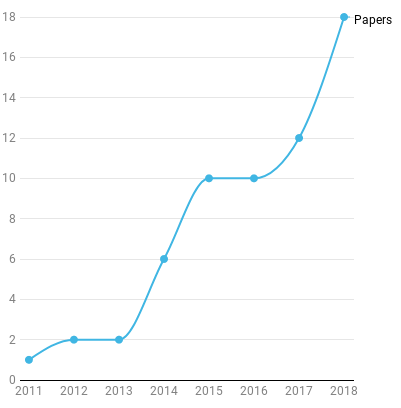
\includegraphics[width=0.45\textwidth]{Pictures/years.png}
    \caption{Papers distribution over the years}
    \label{fig:years}
\end{figure}
%//www.datawrapper.de/_/CHIG7/

CPP has become a compelling topic in latest years, as presented in Figure \ref{fig:years}. During 2018, a total of 18 papers met the inclusion criteria, which is an increment of 33\% compared to the previous year. This shows a rapid increase since the CPP was formulated in 2012. Also, it has attracted interest from several institutions, located mainly in industrialized countries. USA and China are where most of the studies have been developed. Figure \ref{fig:location} presents a map with pointers located on the institutions to which the first author of the selected papers is affiliated. 

\begin{figure}
    \centering
     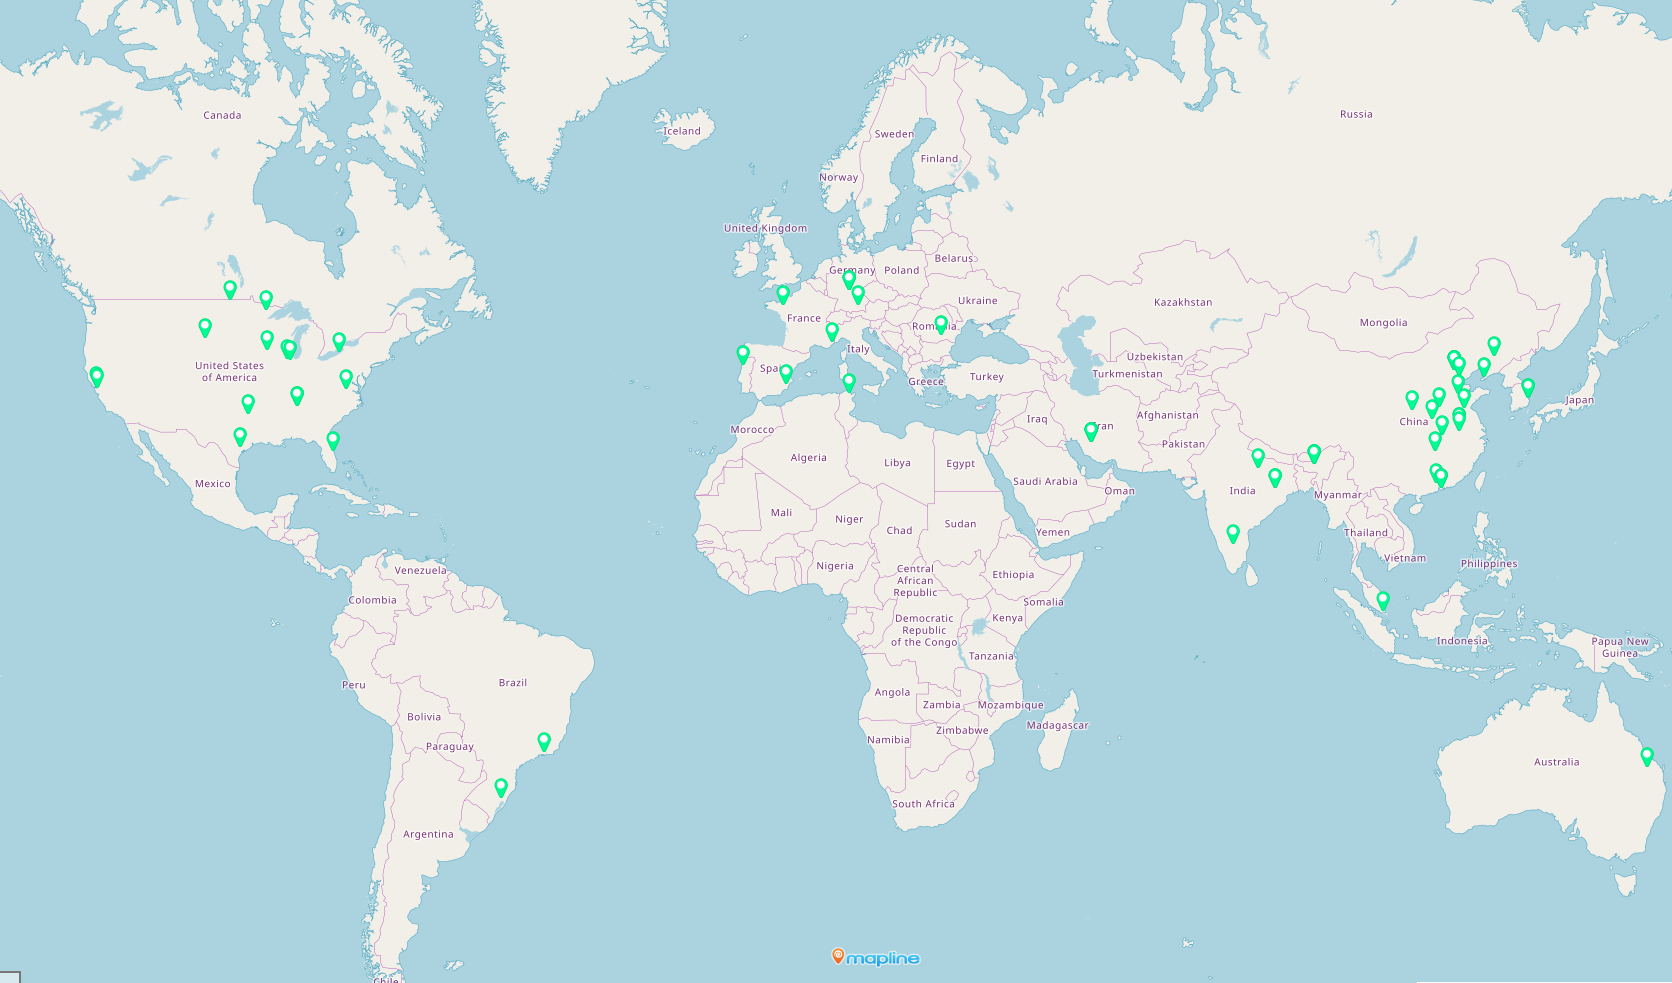
\includegraphics[width=0.45\textwidth]{Pictures/locations10dic2018.png}
    \caption{Distribution of first author's affiliation \dia{How did you know the main author?}\juli{I change it to first}}
    \label{fig:location}
\end{figure}
%https://app.mapline.com/map/map_448677df#

%I comment this figure since is the same info as the following.
%\begin{figure}
 %   \centering
  %  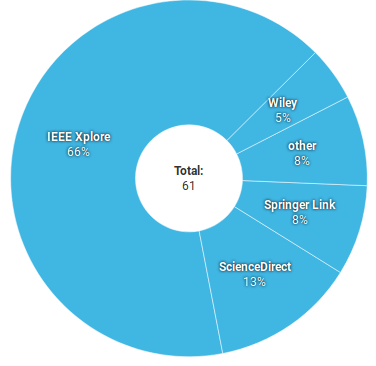
\includegraphics[width=0.45\textwidth]{Pictures/database.png}
   % \caption{Quantity of papers distributed by type and name of the venue}
    %\label{fig:database}
%\end{figure}
%//www.datawrapper.de/_/sPC2v/


% https://www.datawrapper.de/_/ELg2O/
%https://app.datawrapper.de/chart/rC82d/upload

Out of the 61 papers, 66\% (40 works) were published on IEEE Xplore, and 75\% of those are conference papers, as presented in Figure \ref{fig:typevenue}. On the other hand, 38\% of the papers (23 works) were published on different journals, while conferences published the rest 62\%. It is noteworthy that papers published in journals presented a more detailed description of the work. Regarding the conferences, we identified a dificulty to identify the tools and experimental setup for the evaluation of the proposed solution. We consider it was due to the space limitation usually related to this type of publications.


\begin{figure}
    \centering
    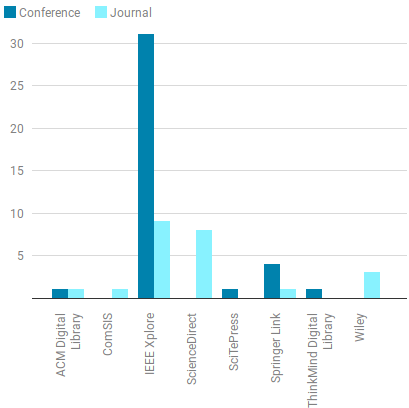
\includegraphics[width=0.45\textwidth]{Pictures/venuesvstype.png}
    \caption{Quantity of papers per type and database\dia{the sum is 51 not 52}}
    \label{fig:typevenue}
\end{figure}

%\subsection{Approach}
%\begin{itemize}
%\item Presenting the SLR
%\item Keywords and research scope
%\item Article selection, inclusion and exclusion
%%\item Questions
%\end{itemize}
%\subsection{Questions to answer}
%\subsection{Main results}
%Quantitative presentation 
%%figure sur les années
%%Stats pour les papiers selon la critère optimisée et l'année

\section{Discussion Addressing Research Questions}

This section discusses the objectives and challenges faced by the collected research papers addressing the CPP. It is organized in the same order as the defined research questions and aims to propose different classifications of the analyzed works by answering the questions.

\subsection {RQ1: What are the purposes of solving the CPP?}
%Intro

In this section, we classify the papers selected to be part of the study as a result of the SLR methodology. The classification categories correspond to the criteria used to select the optimal location for the controller(s) in an SDN, that is the objective function optimized in the CPP. Among each of these classifications, the papers are also categorized based on the optimization problem constraints.

We have identified seven optimization objectives to classify the papers: Latency, Resilience / Reliability, Cost, Number of controllers, Load balance, Power  consumption in addition to Multi-objective criteria. Figure \ref{fig:pyramid_purposes}\fia{why having a 3D figure, do we have something in theb other axe? or we would have the same info with a triangle?} \juli{I thought it look nice :p, already change it} shows the quantity per each category, while Table \ref{tab:category} presents the list of reference per category. We will present the objective and constrains according to the categories.
\subsubsection{Latency}
Latency is one of widely used performance metrics in computer networks \cite{SiHa15}. It is defined as the delay that occurs in data communication over a network. In SDNs, frequent message exchanges between switches and controllers and between different controllers (if there are many) are essential to carry out most SDN functions, such as flow instantiation, state update, etc. Thus, network latency is an important criterion to take into consideration when optimizing SDN networks, namely when optimizing the controller placement. The overall latency consists of packet transmission latency, propagation latency, switch queuing latency, and controller processing latency \cite{WaZh17}. The packet transmission latency is related to the packet size and the data-rate of the link. The propagation latency is proportional to the distance between two communication nodes. The switch queuing latency is the delay caused by a link congestion. The controller processing latency consists of the delay affected by the controller load. However, most of the works presented in the literature to solve the CPP investigate the case of Wide Area Networks (WANs), where only propagation and processing latencies dominate because of the relatively small control message size in SDN and the assumed large capacity of control links. 
\subsubsection{Multi-objective}
When several performance metrics are considered, there is usually no single best controller placement solution, but a trade-off between these metrics. For this, several papers present the CPP as an optimization problem with multi-objective function, that tries to find the best trade-off between the optimized metrics.
\subsubsection{Resilience and Reliability}
There are several definitions of resilience which differ more or less in their meanings. In the following, we shall adopt the definition proposed by \cite{StHu07}, which claims that "resilience is the ability of the network to provide and maintain an acceptable level of service in the face of various faults and challenges to normal operation."  Any other sense considered in the contributions will be pointed out. On the other hand, the reliability of a network is a measurement of the probability of the network to be operative during a period. This, in turn, is a condition to obtain reliability\fia{Not clear to me, reliability is a measurement of the reliability?} \juli{I change it}, which is highly dependant on the controller's ability to stay operative. The studied papers use connectivity as a mean to maintain the network operative.\fia{I dont understand this last sentences.}

\subsubsection{Cost}
In our research, we found that 15\% of the total \mia{reviewed} papers \mia{have as objective} \mia{a given} cost. Some approaches \mia{state} specifically CAPEX and OPEX \mia{reduction objectives}, while others use generic metrics. We included both approaches into the same category, considering that all can translate to economic cost. 

\subsubsection{Number of controllers}
Some works found in the SLR were directed to the reduction of controllers. It is an interesting objective with implications in cost and management  reduction\fia{why would reducing the number of controllers reduce the latency?!}\juli{fixed!}, but an increase in latency. 
\subsubsection{Load Balancing}
In \mia{the} SDN context, the \mia{controller's} load is usually associated with the number of switches connected to a controller. However, there are other considerations also related to load balancing such as control messages \mia{usually referred so as} overhead, that can share the category. 
\subsubsection{Power consumption}
We could include power consumption reduction in the cost category. However, we chose to maintain it separately although it has a single study since it is an interesting approach with environmental implications.
\begin{figure}
    \centering
    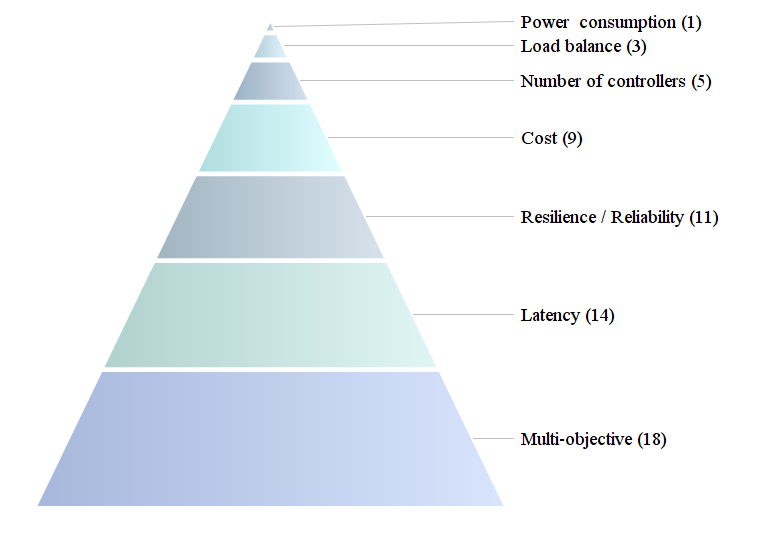
\includegraphics[width=0.45\textwidth]{Pictures/categories.png}
    \caption{\mia{Answer to R1 summary:} Objective functions for the CPP}
    \label{fig:pyramid_purposes}
\end{figure}
% image: https://www.onlinecharttool.com/graph


\begin{figure}
    \centering
    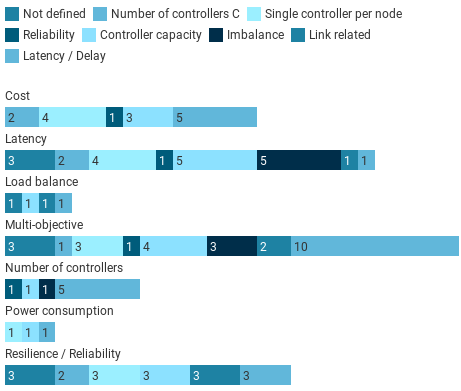
\includegraphics[width=0.45\textwidth]{Pictures/constraints.png}
    \caption{Constraints per category}
    \label{fig:constraints}
\end{figure}
\fia{Is this figure updated? Im not sure we have that much of multi-criteria papers}

% https://www.tablesgenerator.com/latex_tables#

\begin{table}[!h]
    \centering
    \begin{tabular}{l p{5 cm} }
    
  \hline
Category  & Papers        \\  \hline
Cost                     & \cite{11-BaRo13}, \cite{HeBa17}, \cite{RaRe14}, \cite{RoRu14}, \cite{SaHi17}, \cite{SuHa17}, \cite{WuCh18}, \cite{YaHo15}, \cite{ZhWu17}                                                                                                                                       \\
Latency                  & \cite{AlAy17}, \cite{ChCh18}, \cite{GaWa15}, \cite{HeSh12}, \cite{HuLu16}, \cite{KiRa16}, \cite{KiRe18}, \cite{KsBa16}, \cite{MoNa18}, \cite{SaSa16}, \cite{SaSa17}, \cite{WaZh17}, \cite{XiQu14}, \cite{YaBi14}                                                               \\
Load balance             & \cite{HuJo15}, \cite{LiYo16}, \cite{WoLi15}                                                                                                                                                                               \\
Multi-objective          & \cite{AhJa15}, \cite{GoGi17}, \cite{HoHa13}, \cite{JaKe18}, \cite{JiCe14}, \cite{KhAh18}, \cite{KsBa16b}, \cite{KuYi18}, \cite{LaGe15}, \cite{LaGeb15}, \cite{PeRe16}, \cite{TaMo18}, \cite{TaYi18}, \cite{TiZh18}, \cite{VaMo18}, \cite{VoBo15}, \cite{ZhGi17}, \cite{ZhWa18} \\
Number of controllers    & \cite{23-LiWa15}, \cite{26-ChWa15}, \cite{AbMa17}, \cite{SuMa18}, \cite{TaSa18}                                                                          \\
Power consumption        & \cite{HuLu17}                                                                                                                                                       \\
Resilience / Reliability & \cite{FaXi18}, \cite{HuWa12-1}, \cite{LiJia16}, \cite{LiSh18}, \cite{MaDu16}, \cite{MaJe18}, \cite{MuOl14}, \cite{SaSo18}, \cite{VaPo17}, \cite{ViMa16}, \cite{ZhBe11} \\ \hline                                                 
\end{tabular}
    \caption{Papers classification per objective category}
    \label{tab:category}
\end{table}

\subsubsection{Constraints of the optimization problems}
Regarding the constraints, we identify six types: 
\begin{enumerate}
    \item Latency/Delay: maximum value of latency for a specific parameter.\fia{I dont understand "for a specific parameter"}
    \item Number of controllers: maximum quantity of controllers in the network;
    \item Imbalance: bound on the difference of switches assigned to a controller, usually computed as the maximum number of switches assigned to a controller and the minimum;
    \item Single controller per switch: each switch can be associated to a single controller;
    \item Link related: several conditions related to the state of the links between switches and controllers;\fia{can we specify a little bit more?}
    \item Controller capacity: internal capacity of each controller: \mia[]{usually related to the number of flows a controller can handle, or the number of switches it can control}; and
    \item Reliability: maintain a level of reliability in the network.
\end{enumerate}
However, we found a challenge during the revision, since some papers did not state the considered constraints explicitly. To allow the systematic review, we added an artificial type of constraint called \textbf{not defined}. \fia{can we have a table with this classification?}

The paper in the category \textit{Power consumption} presents the constraints \textit{Latency / Delay, controller capacity} and \textit{single controller per node}.
In the category \textit{load balancing}, we found the constraints \textit{controller capacity, link related} and \textit{latency}. \delia{Each, only once  in the three papers of the category.} However the study in \cite{WoLi15} was included in the \textit{not defined} denomination.
Every study on the \textit{number of controllers} category uses the \textit{Latency / Delay} constraint, but also \textit{reliability, Controller capacity} and \textit{imbalance} are present. 
Regarding \textit{Cost} purposes, we found constraints related to \textit{number of controllers, single controller per node, reliability, controller capacity} and  \textit{Latency / Delay
}. The latter was the most common, found in five different papers. The least common is \textit{reliability}.
For the category \textit{Resilience / Reliability}, the excluded constraints were \textit{imbalance} and \textit{reliability}. The included ones have an almost uniform distribution. 
For the category \textit{latency} we presented fourteen works, and we identified that all the defined types are present, but the most recurrent are \textit{controller capacity} and \textit{imbalance}, followed by \textit{single controller per node}. The least common constraints are \textit{link related, reliability, number of controllers} and \textit{latency}. For the latter case, the constraint considered a different measurement of latency. Finally, we found three papers \cite{SaSa17,WaZh17,HeSh12} that did not state clearly their constraints.
\textit{Multi-objective} category, being the largest, has most of its constraints in the \textit{Latency / Delay} denomination, since ten out of its eighteen papers use it. The other constraint denominations are also used, to a lesser extent. The studies in \cite{AhJa15, HeSh12, HoHa13} did not specify the constraints. Within this category, we identify a rare consideration in the study \cite{TaMo18} regarding time, since it presents an incremental location of the controllers, depending on the period.
\fia{it would be nice to clearly state (figure or table) the different "latencies" considered by papers: switch-controller, intercontroller and worst case, average, all being propagation latency} \juli{I plan to do that in the RQ6 for the metrics}

The broadest category is multi-objective, which answers to the real situation of a network that requires several trade-off performance criteria. In 2018 there was a trend to the multi-objective category since 50\%  of the studies fell in it. However, Latency and Resiliency / Reliability, and cost remain relevant objectives with significant percentages of the papers in the last two years. 

\fia{we need a transition here} \juli{do you mean a sentence like this one??}
In the next section, we will study the proposed methods to solve the optimization functions.


\subsection{RQ2: \modia{Which methods are} used to solve the CPP?}

Both exact and heuristics methods have been proposed for the CPP and, for several works, there is a comparison between techniques that used both methods. 

For the classification into exact or heuristics, we selected the specific method used for locate the controller. This distinction is important because there are procedures (such as partitioning the network) that require a different algorithm. 
We classified the papers into two categories:
\begin{enumerate}
    \item Exact: Studies that declare to find an optimal solution
    \item Heuristics: Studies that used a heuristic method or stated to find a sub-optimal (near-optimal) solution.
\end{enumerate}

Approximately 13\% of the \mia{reviewed} works, use the two of them for comparison purposes. In these cases, exact methods are proposed usually as a starting point, and authors propose to use heuristic methods that reduce the computing time for the solution. 

Over 64\% of the reviewed papers (39 studies) decided to use a heuristic approach. Out of that amount, 8 papers used both an exact and a heuristic approach. 
Several authors proposed an algorithm with their own technique, and the rest used varied options such as:
\begin{enumerate}
    \item Genetic
    \item Greedy
    \item Simulated annealing
    \item Graph theory \juli{I dont know if it is a suitable classification, please check}
    \item Swarm 
\end{enumerate}

On the other hand, exact methods were used in 47\% of the reviewed papers (29 studies) and the techniques identified are listed below:

\begin{enumerate}
    \item Game theory: bargaining games and non-zero-sum game.
    \item Programming: integer linear programming, mixed integer linear programming, integer quadratic programming, and binary integer programming.
    \item Exhaustive search
    \item Triangulation: Bowyer-Watson algorithm
programming. 
\end{enumerate}

Several authors proposed to continue their research with heuristic algorithms. 

The paper \cite{TaYi18} presented the problem formulation and results of the simulation. However, it did not presented the method used to solve it. 

\begin{figure}
    \centering
    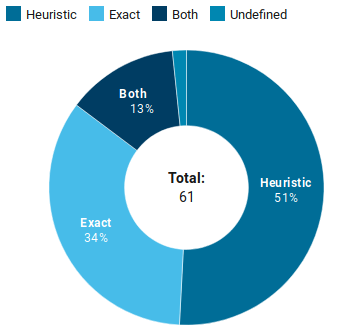
\includegraphics[width=0.45\textwidth]{Pictures/approach_Heur_exact.png}
    \caption{Approaches to solve the CPP}
    \label{fig:approach}
\end{figure}

\begin{figure}
    \centering
    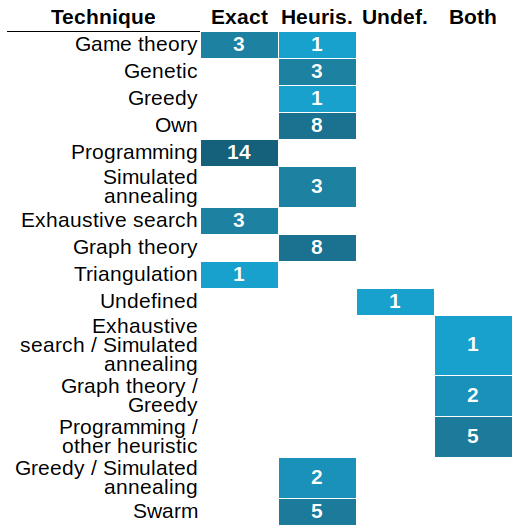
\includegraphics[width=0.45\textwidth]{Pictures/tecnique_method.png}
    \caption{Type of algorithms vs approach used to solve the CPP}
    \label{fig:type_algorithms}
\end{figure}

\begin{figure}
    \centering
    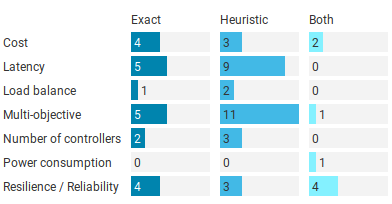
\includegraphics[width=0.45\textwidth]{Pictures/category_method.png}
    \caption{Approaches to solve the CPP per category}
    \label{fig:approach_cat}
\end{figure}



 

\subsubsection{Mathematical programming} \fia{mathematical programming?} Out of all the presented methods, integer programming is the one that groups the majority of the solutions for the CPP. Within this category, there are also different techniques such as integer linear programming, mixed integer linear programming, integer quadratic programming, and binary integer programming. In \cite{HeBa17}, the authors used nonlinear programming along with MILP, which is solved with a python-based framework \delia{is implemented} and Gurobi.


\subsubsection{Clustering} Another popular method to formulate the CPP uses the k-center and k-means in graph theory. It is, however, an NP-hard problem. In half of the works in the section, the authors propose exact algorithms to solve the problem. However, heuristics are preferred, because of the computational complexity.


\subsubsection{Particle Swarm Optimization}
%GaWa15, SaSa17, 23-LiWa15

\subsubsection{Genetic}
%AhJa15, VaMo18

\subsubsection{Simulated annealing}
%MaDu16 MaJe18

\subsubsection{Game theory}\fia{This is not the solution but the model}
%KsBa16, RaRe14, KiRe18. It has both heuristics and exact methods

\subsubsection{Pareto}
%LaGeb15, HoHa13, KsBa16b. It has both heuristics and exact methods
The different parameters and requirements of the network present trade-off's that must be addressed.  The Pareto optimality 


\subsection{RQ3: How are the methods evaluated?}

Every paper we reviewed informs the specific topology or at least their source. 60\% of the studies (37 papers) obtain the used topologies from the Topology Zoo \cite{topologyzoo}. 

SDN-Lib \cite{sdnlib} is the source of 5 papers, while Rocket Fuel repository \cite{rf} is used on 3 studies. nsfnet is used in 2 papers. 

17 papers use only one topology and the sources are: Abilene, Internet 2 OS3E (4 papers), Iridium, NSFNET, a single topology from the Topology Zoo (4), 1 random topology, and 5 papers that used their own topology.



\begin{figure}
    \centering
    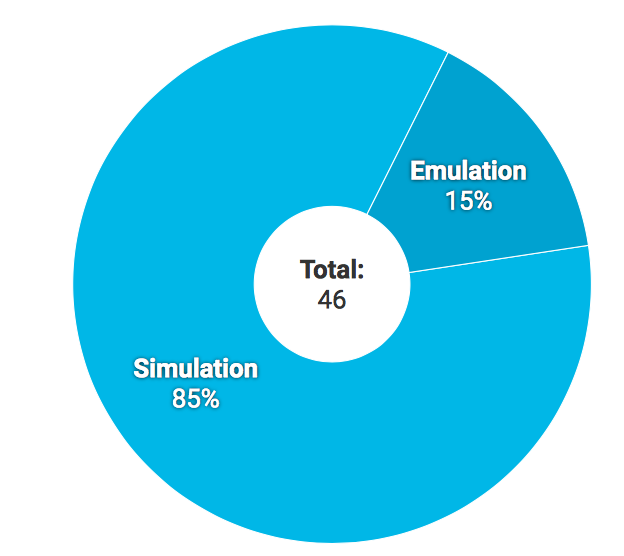
\includegraphics[width=0.45\textwidth]{Pictures/Test nature.png}
    \caption{Test nature}
    \label{fig:test_nature}
\end{figure}

\begin{figure}
    \centering
    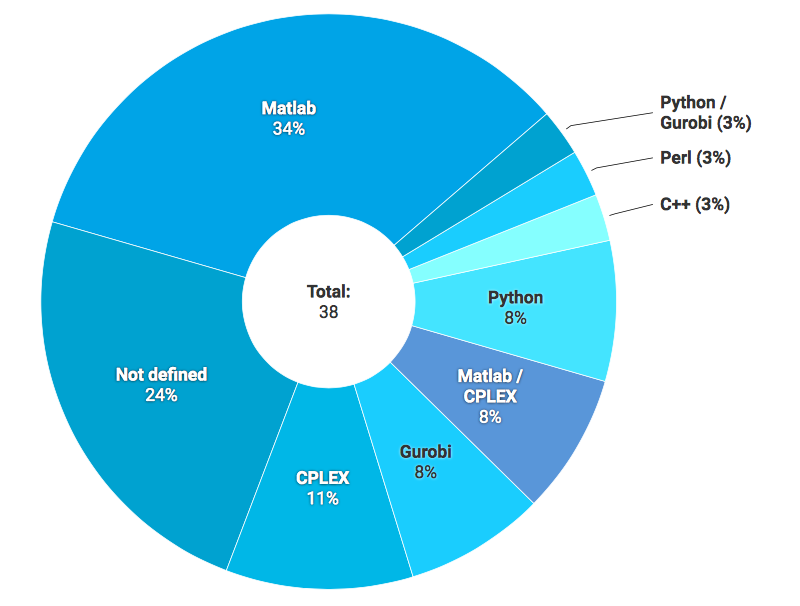
\includegraphics[width=0.45\textwidth]{Pictures/Simulations.png}
    \caption{Tools used for simulation}
    \label{fig:simulation}
\end{figure}

\begin{figure}
    \centering
    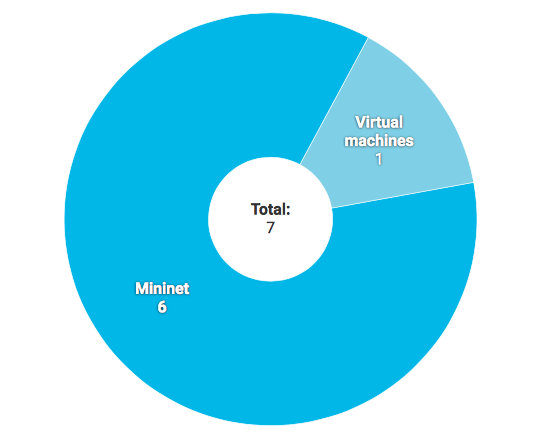
\includegraphics[width=0.45\textwidth]{Pictures/Emulations.png}
    \caption{Tools used for emulation}
    \label{fig:emulation}
\end{figure}



\subsection{RQ4: What are the experimental setup to evaluate the test scenarios?}

Evaluation of the proposed solutions was made either with a simulation or an emulation. In a few cases \cite{LiYo16,GoGi17,BaRo13} both approaches are used, but the majority of the papers use only one. The distribution of papers per test nature is presented in Figure \ref{fig:test_nature}. Only 15\% of the proposals emulate a network either using Mininet or Virtual Machines, as presented in Figure \ref{fig:emulation}.

On the other hand, most of the papers use a simulation approach, for which they employ several software tools. Matlab is the most extensively used (42\%) followed by CPLEX (19\%). A total of 8\% of the papers used both of these tools. Gurobi solver and Python language are next in the scale, each with a 9\% of use. Finally, we found one simulation with Perl and another with C++.

Simulation, emulation or testbed (planetlab).

\begin{figure}
    \centering
    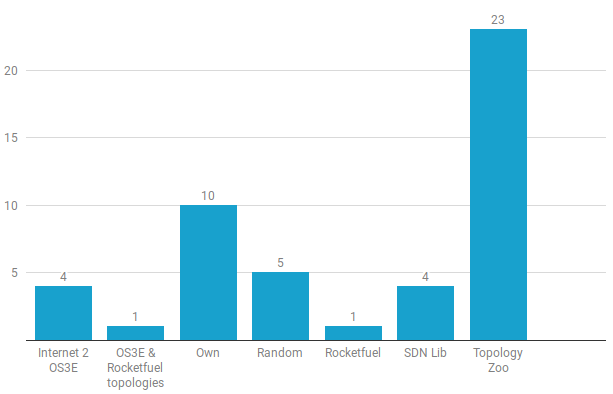
\includegraphics[width=0.45\textwidth]{Pictures/topologysources.png}
    \caption{Sources of the topologies used in the different papers}
    \label{fig:top_source}
\end{figure}
%//datawrapper.dwcdn.net/9O2Nv/1/

\begin{table}[!h]
  \centering
\begin{tabular}{l p{3.2cm} p{3.6cm} }
Topologies used & Reference \\
1 & \cite{AhJa15,RaRe14,WaZh17,HuJo15,SaHi17,XiQu14,LiYo16,SuMa18,ZhGi17,MaJe18,VoBo15,ZhWu17} \\
2 & \cite{BaRo13,WoLi15,FaXi18,AlAy17,YaHo15,HeBa17} \\
3 & \cite{HuWa12,MuOl14,MaDu16,KiRa16,SaSa16} \\
4 & \cite{HuLu17,ZhBe11,KiRe18} \\
5 & \cite{ViMa16} \\
10 & \cite{HuLu16} \\
16 & \cite{AbMa17} \\
20 & \cite{SaSa17} \\
24 & \cite{PeRe16} \\
40 & \cite{VaMo18} \\
60 & \cite{LaGe15,LaGeB15} \\
74 & \cite{ChWa15} \\
82 & \cite{YaBi14} \\
124 & \cite{RoRu14} \\
140 & \cite{HoHa13} \\
Not,defined & \cite{LiWa15,KsBa16,LiJia16,GaWa15,KsBa16b,VaPo17,GoGi17} \\
Over,200 & \cite{HeSh12,JiCe14,SuHa17}
\end{tabular}
\caption{Number of topologies used per paper}
    \label{tab:topologies}
\end{table}


\subsection{RQ5: What are the case study assumptions?}
Topologies. (merge with RQ3?)
\fia{I would put static or dynamic as an answer to this question, also, specify the scenario: WAN, Datacenter, 5G networks, etc. I would put topology as an answer to question RQ3}

\begin{figure}
    \centering
    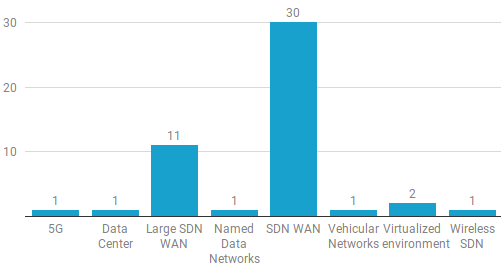
\includegraphics[width=0.45\textwidth]{Pictures/scenario2.png}
    \caption{Scenarios for the CPP}
    \label{fig:Scenarios1}
\end{figure}
%//www.datawrapper.de/_/E7qyM/


\begin{figure}
    \centering
    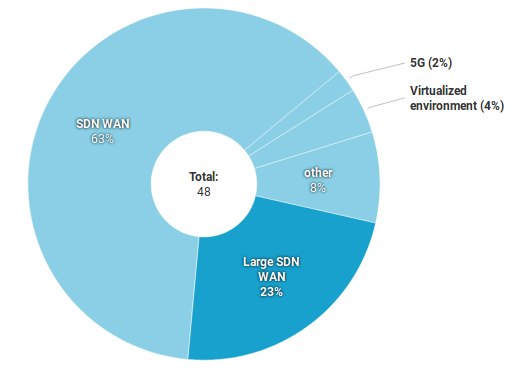
\includegraphics[width=0.45\textwidth]{Pictures/scenario1.png}
    \caption{Scenarios for the CPP}
    \label{fig:Scenarios2}
\end{figure}
%//www.datawrapper.de/_/E7qyM/
%//www.datawrapper.de/_/SP9In/

Regarding the scenarios in which the CPP was formulated, we found eight categories: 

\begin{enumerate}
\item SDN WAN
\item Large SDN WAN
\item 5G
\item Data Center
\item Named Data Networks
\item Virtualized environment
\item Vehicular Networks
\item Wireless SDN
\end{enumerate}

The majority of the studies were explicitly for WAN or did not indicate any particular assumptions, but we were able to identify it with the topologies used for testing and then classify it in categories 1 or 2. For this distribution, we considered that large SDN WAN refers to scenarios with 40 or more switches. Only papers with a specific application (categories 3 to 8) referred to a distinct scenario. This situation was identified in 14\% of the papers, as presented in figure \ref{fig:Scenarios2}. 

We also identified the requirement for a dynamic or static calculation of the CPP, depending on the time taken to compute the solution. We consider that dynamic solutions consider changes in the network status and require short time for convergence. Static approaches only considered a single calculation to operate the network or cannot respond to sudden changes in the network. 

Categories 3 to 6 presented dynamic solutions, while categories 7 and 8 presented only static considerations. On the other hand, the papers for WAN scenario (86\%) had a distribution of 27\% for dynamic and 73\% for static configuration. The distribution is presented in figure \ref{fig:Scenarios3}. 

\begin{figure}
    \centering
    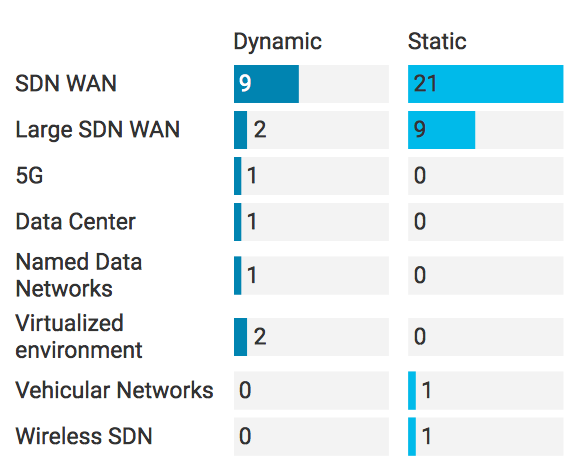
\includegraphics[width=0.45\textwidth]{Pictures/Scenarios3.png}
    \caption{Categories of scenarios and requirement for dynamic/static calculation}
    \label{fig:Scenarios3}
\end{figure}







\subsection{RQ6: What are the metrics evaluated by the proposed work?}
What metrics are evaluated for each proposed scheme? (Nb of controllers, latency, connectivity loss).


\section{Prospective Research}
\begin{itemize}
\item Real analysis with real traffic
\item Distributed control plane design
\item Apply to use case
\end{itemize}

\section{Conclusion}
\medskip
\tableofcontents

\bibliographystyle{unsrt}%Used BibTeX style is unsrt
\bibliography{bib_survey}
\appendix

Papers' summaries. \fia{The text below was in the RQ1 section, I've just moved it here, we might not include it in the final version of the paper.}


\subsubsection{Latency}
In this section, we present the papers summary % solutions to the CPP by minimizing the propagation latency between switches and controllers as well as inter-controllers latency. Other works that minimize the propagation latency along with processing latency are also presented.}

The first statement of the CPP was presented in \cite{HeSh12} by Heller et al., and the approach was influential for the subsequent proposals. The authors evaluated optimal placement using brute force, directly measuring the defined metrics on all possible combinations of controllers on WAN networks\fia{can we say on how many networks?.} selected from Topology Zoo\fia{reference?}, using Matlab. \mia{These defined metrics were switch-to-controller latency, considering both average latency --averaging across all switches in the network-- and worst switch-to-controller latency}. Results showed that the location and \mia{optimal} number of controllers depend on the simulated network's topology. They also note that the average latency with a random placement is $1.4$ to $1.7$ larger than that of the optimal placement, while this ratio is between $1.4$ and $2.5$ for worst-case latencies. \delia{The work consider the switch-to-controller latency and propose exhaustive research to find the optimal placement by directly considering the metrics on all possible combinations of controllers.} \mia{The problem of minimizing} \delia{Both} average and worst-case latencies \mia{is formalized as }\delia{are minimized by investigating} k-median and k-center problems, respectively. 

\delia{The a} \mia{A}verage latency metric \mia{--either switch-to-controller or inter-controller--}\fia{verify that this is correct} is considered in several works \cite{SaSa16, GaWa15, SaSa17, AlAy17, HuLu16, XiQu14, KsBa16}, \mia{while} fewer papers \cite{YaBi14, KiRe18} focus on the worst case latency approach, as presented below.

%---------

In \cite{WaZh17} a survey on the controller placement problem is presented. The authors draw a taxonomy based on the objectives of the research works in this field. Models, objectives and solutions are elaborated for each category. This paper also proposes an algorithm to address the controller placement problem in the aim of minimizing the maximum latency between controllers and switches. The proposed approach, called Clustering-Based Network Partition Algorithm, iteratively partitions the network into different subnetworks. For each subnetwork, a centroid that has the minimum sum of physical distances to all nodes is selected. %The performance of the proposed algorithm is evaluated in comparison to the k-center and k-means approaches. The Internet2 OS3E topology was chosen, where the nodes coordinates were obtained from Google Map and the distances of the links were calculated using the "haversine" formula. The shortest path distance was calculated using Dijkstra's algorithm. Simulations show that the proposed approach ensures smaller maximum latency between the controller and associated switches than the one achieved by both k-center and k-means. 

The global average propagation latency ,i.e. the sum of switches to controllers latency and the inter-controllers latency, is minimized in \cite{SaSa16}. It is calculated as the sum of switch-to-controller and inter-controllers distances. The authors propose a spectral clustering algorithm that partitions the network into smaller domains based on the distance between nodes, to optimally place the controller within the domain. The proposed constrain is no node or edge can allocate to more than one sub-graph, which is the same as to have a single controller per node. This specific objective is widespread, and other works\fia{can we provide references} have used it too. 

One of them is \cite{SaSa17}, where the authors use controller-to-switch latency and inter-controller latency as the optimization metrics\fia{is it the sum of both?, if so we should say it to avoid confusion with multi-objective} with the objective of minimizing the average value. Two population-based meta-heuristic approaches were proposed: Particle Swarm Optimization (PSO) and Firefly. The PSO approach considers two types of learning (i.e., social and cognitive), while the Firefly approach considers the bio-luminescence biochemical process. % Each approach generated an algorithm, and they were tested on 20 elements of the Topology Zoo, presenting TataNId topology as an example. It has 144 nodes and 141 edges. Results show Firefly That approach is better than PSO regarding average and worst-case latency and it converges slightly faster than PSO.

Mentioned works optimized the propagation latency without taking into consideration any other performance metric. However, we found that most of the papers that considered latency, also included a constraint related to load balancing, aiming to select proper capacity to each controller.

Yao et al. \cite{YaBi14}  introduced the capacitated controller placement problem (CCPP), which objective is to minimize the maximum worst-case\fia{maximum is not the same as worst-case?} latency between the switches and their assigned controller, subject to the controller capacity. In their model, the controller load is calculated by the processing of PACKET\_IN events, delivering the events to the applications, communicating with other controllers and maintaining the view of the local network partition. \mia{Such controller load} \delia{It} has to be maintained under a \mia{given} capacity limit. %The problem being NP-hard, a capacitated k-center strategy based on the algorithm introduced in \cite{OzPi06} is proposed to solve it. An Integer Programming model is also used to find the minimal number of controllers with a specified radius, where the radius denotes the maximum propagation latency between switches and the assigned controller. According to simulations, the proposed strategy can reduce the number of controllers required to avoid overload as well as the load of the heaviest-load controller, when compared to the k-center algorithm.  %Also, it has smaller radius than using dynamic controller provisioning or dynamic scheduling strategy in k-center placement.

The controller capacity is also considered as a constraint in \cite{GaWa15} but the objective is to minimize the average global propagation latency, considering also the number of controllers as constrain. The authors propose a particle swarm optimization (PSO) algorithm to solve the problem. %However, the evaluation of the proposed algorithm is not very clear since it is based on the comparison with other algorithms solving different objective functions. 

In \cite{HuLu16} authors address the CPP with the objective of minimizing both\fia{the sum of?} average and worst case latency but considering the load of the controllers as a constrain that represents a trade-off. It also considers a defined number of controllers. For that, a Binary Integrer Programming technique is presented. 

Additionally, in \cite{AlAy17} the objective is to minimize two\fia{the sum of?} metrics that present a trade-off: the intra-domain and inter-domain latency. The constraint considered relates only to assigning all switches to a single controller. %For this, the article formulated an ILP, wich was not solved due to its complexity. Instead, two clustering algorithms were proposed. The results showed significant improvements regarding latency in downloading data and average performance.

In \cite{KiRe18}, authors present a game theoretic approach with two algorithms to attend the main goal of network partitioning. the first algorithm "Network partitioning" seeks to partition the network into sub-networks as initialization. The second algorithm "Cooperative k-means network partitioning" is modeled as a cooperative game.\fia{Im not sure I understand, the problem is modeled as a cooperative game, not the algorithm, right?} Switches try to form coalitions with other switches to maximize their value. The work presents the worst case \mia{latency} as metric.\fia{switch-to-controller propagation latency, right?}

In \cite{KsBa16}, authors present three perspectives for the optimal location of the controller, that consider as metric the overhead in the communication: i) CCA (Controller-Controller communication overhead Aware solution), ii) SCA (Switch Controller Aware communication overhead solution), and iii) FTCS (Faire optimal Tradeoff Between CC and CS communication overhead solution) which uses the \delia{theory} Nash Bargaining \mia{solution} \delia{game} to ensure the balance between the two methods previously (CCA and SCA). FTCS becomes an optimization problem, where metrics are based on the overhead of the communications. %These proposed solutions were tested using IBM CPLEX, Matlab and CVX 2.0, which concluded that the solution helps to minimize latency and overhead while ensuring load balancing. %ii) SCA (Switch Controller Aware communication overhead solution), Usually, this parameter is defined by the network operator, according to the link between bandwidth and traffic handled by different switches.

The worst-case \mia{switch-to-controller} latency is \mia{also} \delia{a metric} reviewed in \cite{XiQu14}. \delia{It} \mia{Authors} propose the spectral clustering method to divide a WAN-SDN topology into several small domains, and the CPP solution seeks low latency, load balancing between controllers, and high reliability for each cluster, which is a differential element with all the other proposals. Both reliability and load balancing are presented as constraints. \delia{Metrics location problem of SDN controller were defined to minimize propagation delays while ensuring load balance and ensures the reliability of the controller.} The problem is modeled as a binary integer problem (BIP), with a static controller.\fia{what is a static controller? shouldn't we specify?} %Software CPLEX optimizer is used to evaluate the increase in latency in ten topologies with different sizes of SND-lib to evaluate the model. The experiment results showed that the model could achieve a balanced level control with a small increase in optimal latency. The model is not suitable for large-scale topologies because of the computational requirements.


\subsubsection{Multi-objective CPP}



%POCO, in its default configuration, performs an exhaustive evaluation of all possible placements. Thus, it is practically possible only for small and medium sized networks and cannot be feasible for large-scale or dynamic networks as it has high time and resource constraints such as processing and memory. 

Authors in \cite{LaGeb15} propose a heuristic solution for the CPP with short computational time, aimed to be used in a dynamic environment. The solution considers a particular set of optimization objectives and returns the possible trade-offs between them. The criteria for the problem are latency and imbalance. The former is defined in two ways: the average node to controller latency calculated as the shortest path, and the average node to controller latency specifying any controller\fia{"specifying any controller" I dont understand this!}. The latter criterion uses the imbalance metric, which captures the difference of the total number of nodes assigned to the controllers with highest and lowest amounts.

 
%. The authors derive guidelines for deciding whether to use an exhaustive evaluation or to switch to an heuristic approach, according to different use cases and requirements. The heuristic algorithm proposed in this work is based on Pareto Simulated Annealing (PSA), a Multiobjective Combinatorial Optimization (MOCO) algorithm inspired by simulated annealing. The heuristic method analyzes the trade-off between the time and accuracy and takes the latencies of the nodes, the latencies between the controllers, failure tolerance in nodes , failure tolerance in links and the load balance. Simulation results show that this method is less precise but faster to determine the location of the controller.
The work in \cite{LaGe15} introduces a framework to solve the CPP which evaluates all the possible scenarios. Since brute force approach is not appropriate for large-scale networks, the authors propose a heuristic approach with a simulated annealing algorithm. For this, they define a set of criteria that includes latency, both average and maximum for node-to-controller and controller-to-controller. It also considers resiliency for failure tolerance when the link node-to-controller fails by using a metric for the imbalance, i.e., the difference in the total number of nodes assigned for a controller, for the two controllers with the lowest and highest amount of assigned node\fia{I dont understand how this means resiliency}. As a result, there are five criteria to have into account for the placing algorithm, which speedups\fia{speeds up with respect to what?} computation beyond a factor of 20, depending on the required accuracy. In \cite{LaGe15}, the authors extend the research into the heuristic methods and add the criterion of the number of controller-less nodes when a failure occurs.

Other works try to solve the multi-objective problem for large-scale networks, by proposing heuristic schemes and using the criteria proposed by \cite{LaGeb15}. In \cite{AhJa15} Ahmadi et al. proposed a genetic algorithm called Hybrid NSGA - II. This genetic algorithm is normally used in discrete and continuous optimization problems and this model is applied to the controller location problem. NSGA-II demonstrated the efficiency when require\fia{while requires?} high computational effort and processing time during the test. The algorithm has good performance also in cases where the network needs to adapt to changes, and even efficient large-scale networks.
% In \cite{JaAh15}, another heuristic extension to POCO based on NSGA-II (Non-dominated Sorting Genetic Algorithm II)  mixed with Pareto Frontier is proposed. This genetic algorithm is normally used in discrete and continuous optimization problems and this model is applied to the controller location problem. Latency between switches and its assigned controllers, inter-controllers latency, as well as load balancing between controllers are considered.
An extension of this work is presented in \cite{JaAh15} that improves the original algorithm to solve the CPP with better performance in larger instances. 


Another example of the use of those criteria is \cite{VaMo18}. In this paper, the authors propose a heuristic algorithm called Multi-Start Hybrid Non-dominated Sorting Genetic Algorithm (MHNSGA) to solve the multi-objective CPP. The proposed algorithm is an adaptation of an NSGA algorithm especially based on greedy initialization and multi-start mechanism. Compared to the framework POCO\fia{not introduced with this name}, the proposed algorithm is able to find near-optimal solutions with much less run time and memory and, unlike POCO, it can be applied to large-scale networks. However, for such large-scale instances, it is not possible to evaluate the accuracy obtained by any heuristic algorithm since we can not calculate the exact solution for the evaluated placements.\fia{can we cite the metrics considered?}%Controller to switch latency, inter-controllers latency, and load balancing between controllers are optimized. Both average and maximum values are considered for latencies.  For smaller network sizes, MHNSGA is compared to POCO over 40 graphs from the Internet Topology Zoo and it is shown to provide an efficient estimation and good convergence towards the real Pareto optimal set. Compared to other heuristics, namely PSA \cite{LaGeb15} and PSO-CGLPP \cite{GaWa15}, MHNSGA converges faster and outperforms the two algorithms in most of the time.  

In \cite{PeRe16}, the authors formulate a ILP for the CPP with two objectives: 1) to minimize the number of active controllers that are needed in a WAN, considering several levels of backup controllers and maintaining latency, capacity constraints and load balancing, and 2) to minimize the worst-case latency between switches and controllers. 
%The proposal was evaluated in topologies issued by SND Lib. In the sensitivity analysis they found that when the probability of failure of drivers is close to 0, the formulation tends to give very little support levels. When the graphics are denser, more possible connections controller-switch and require fewer drivers. The optimal number of drivers depends on the length of the shortest average distance. The number of drivers increases as the maximum latency decreases[USTA]

In \cite{HoHa13}, an exhaustive evaluation of multiple metrics is presented and the resilient Pareto-based Optimal Controller placement (POCO) is introduced. The proposed framework allows to investigate a multi-objective optimization problem, offering all possible solutions evaluated by all objectives, allowing to select afterwards the placement that is most adequate for each one needs. The optimization objectives addressed by the authors are maximum latency between nodes and controllers, inter-controller latency, load balancing between controllers and resilience. For resilience, the authors consider both tolerance on network disruption as well as controller failures. Simulations evince an improvement in calculation times\fia{improvement with respect to what?}, a more efficient use of memory and RAM. The authors extend their work in \cite{HoHa14} where they present the POCO-PLC method applied to the CPP in a dynamic way in SDN networks. Their proposal enables real-time performance analysis, using the PlanetLab network programmed in Python that measures the latency between external nodes and latency between local nodes in real time, as well as the load on the CPU. Then "Planet Lab"\fia{PlanetLab is the test infrastructure, it is not the intelligence choosing the controller} dynamically chooses the controller closest to the node in terms of the latency. Since the controller assignment is dynamic, it allows comparing in real time the different locations of the controller with respect to the previous locations.

A different approach is presented in \cite{ZhGi17}, which considers scenarios for real ISP with multiple controllers. The optimization function aims to minimize the reaction time (defined as the perceived latency by the switch when a new network event is generated) with the following constraints \delia{are}: 1) each controller is placed at only one switch, 2) each switch can host at most one controller, and 3) each switch has exactly one master controller. %The metrics used to solve the CPP are the controller-to-controller and switch-to-controller delay, defined as the time required for the controllers to exchange information and reach a common network state.

A more comprehensive proposal is made in \cite{VoBo15} with an optimization method based on multicriteria decision (MCDA), applicable to the CPP, that can adopt different criteria. The authors present a summary of the standard metrics presented in CPP literature: performance\fia{what is the metric?}, reliability, and latency; as well as their usual constraints. Additionally, they note that the purpose of the paper is not to develop a specific algorithm to find an optimal solution for given criteria; otherwise, to propose a method for overall optimization of the CPP using multicriteria decision. In this case, proponents used some decision variables such as Average Latency, worst latency (Failure-free case), Intercontroller Latency,  each with a given priority. The authors concluded that the method is generic enough to be applied in several stages and internet providers can include resolving the CPP in a specific network. 

A different perspective is presented in \cite{GoGi17}, which considers virtualization of the network. SDN enables virtualization of the network to share the SDN physical network among multiple virtual networks SDN (vSND) each with its own controller. Because resources are finite, physical SDN is crucial to efficiently allocate vSDN applications, known as the problem of integration of VN into a network virtualization environment. The paper presents 2 criteria required to solve the CPP in vSDN: 1) minimizing the embedding cost the VN: mapping the virtual network (VN) requests to specific physical nodes and paths in the physical substrate network (SN) with economical cost metrics; and 2) minimize the average controller-to-switch delay in the SN. \fia{I think this paragrpah is not clear enough, rephrasing is needed}

\delia{The last paper reviewed that presented multi-objective CPP is} \mia{In} \cite{KsBa16b}, an approach of CPP in 5G mobile networks \mia{is presented}. The main concern is to reduce flow installation latency, considering the dynamic environment. The objectives are 1) to minimize the amount of rellocation of the controllers, and 2) to minimize the load of the controller. \mia{The problem is modeled using a Nash Bargainign game from which a Pareto-optimal solution is derived}. \delia{The proposed algorithm uses Pareto optimal trade-off, calculated  with a Nash Bargaining game.}

As presented, most of the multi-criteria objective functions presented aim to improve both latency and \mia{load} balance (or imbalance as defined in \cite{LaGeb15}). Only the works presented in \cite{ZhGi17,GoGi17,KsBa16b} do not consider that combination as objectives. The former includes latency without load balancing. The other two\fia{is it not clear which two} have distinctively different goals (cost related, relocation reduction respectively), probably due to the specific scope they cover (vSDN and 5G mobile networks, respectively).

On the other hand, additionally to latency and \mia{load} balance objectives, \cite{VoBo15, LaGe15, HoHa13, VaMo18} present reliability or resiliency goals, and \cite{PeRe16} includes the number of controllers in the objective function.

Regarding the constraints, \cite{AhJa15,LaGe15, HoHa13} do not specify additional constraints as the embedded in the objective function. \fia{The summary presented in these 3 last paragraphs is nice, can we present it in a chart form?}

\subsubsection{Resilience and Reliability}


Although the CPP was formalized by Heller \cite{HeSh12}, the work in \cite{ZhBe11} which was published one year before Heller's paper, treats the same problem, i.e. controller location, but in the aim to maximize the network resilience. The authors propose a min-cut based graph partitioning algorithm for controller placement to maximize the resilience of the network by minimizing inter-cluster connectivity and intra-cluster difference. Using these two criteria, the authors aim to identify partitions with minimum cuts across boundaries and, subsequently, assign the controller location to the switch with the shortest paths to all switches within the cluster, i.e. the centroid. They consider different types of failures, namely links and nodes failures. Additionally, the partitions are identified with minimum cuts across boundaries, i.e. ensuring a minimum connectivity between clusters. After the partitioning, the controller is placed in the centroid of the partition to guarantee the shortest path length to all switches in the same cluster.% The proposed approach is evaluated using a perl-based simulation tool. Simulations show the impact of controller placement on resilience, and prove that the proposed algorithm outperforms the random and greedy based placements in terms of failure probability in various topologies and that this improvement is more important with large-scale networks. 

The same problem is investigated in \cite{MuOl14}, where the authors propose "Survivor": a resilient framework which reinforces the connectivity between controllers and switches, taking more routes, avoiding the overload of the controller and improving the failover by composing a list of backup controllers for each device in the network. The proposed approach encompasses two phases: Firstly, the CPP is investigated, such that capacity constraints are satisfied and connectivity is maximized, by choosing positions that yield the highest number of node-disjoint paths between the controller and the switches.\fia{And the second phase?} %This method is evaluated with various simulated topologies from Topology Zoo and compared to the algorithm proposed in \cite{ZhBe11}. Many improvements of "Survivor" are noted: (a) considering multiple paths, i.e. exploring path diversity during placement, which reduces the chance of connectivity loss; (b) taking into consideration the capacity to avoid controllers overload; (c) improving smart recovery mechanisms thanks to the proposed heuristic for selecting backups during failover.

Resilience is jointly optimized with switch-to-controller link length in \cite{ViMa16}. In this paper, two strategies for controller placement in the aim of providing protection against link and node failures while minimizing controller to switch latency are proposed. In the first strategy, every node must be connected to its assigned controller over two disjoint paths. In the second one, every node must be connected to two different controllers over two disjoint paths. The main idea of this work is to consider planning of the backups paths in advance. An optimization problem to find a controller placement that jointly optimizes working and backup paths is investigated for the two strategies. %The problem is formulated as a Mixed Integer Linear Programming and the optimal placement is found using the Gurobi solver. %The evaluation of performance metrics in several topologies with tens of nodes shows that the working paths in the proposed strategies may be longer than in the unprotected case (without backup paths). This difference decreases as the number of controllers increases. Simulations also show that both strategies ensure lower control path loss and better control path availability than the unprotected case. The authors verify the feasibility of the solving time for the simulated topologies with single and double link failures. However, they note that this time is not suitable for online use. %However, this paper does not take into consideration the capacity constraints.

Resiliency is also the objective for \cite{MaDu16}. The authors propose a distributed control architecture with clusters managed by independent controllers. Optimization criteria used for this work is i) minimize average latency between controller and switches, ii) maximize resilience by distributing fairly the connections from switches to controller according to the possibility of controller failure. The authors proposed two heuristics to optimize the \mia{controller's} location \delia{of the driver} based on minimizing the likelihood of network partitioning, FairMAx, PartMin, this second stage based on the fair distribution of switches controllers, ensuring network resiliency.\fia{Sentences not clear to me, specially "minimizing the likelihood of network partitioning"}  %The prototype of the proposed controller was implemented in three topologies real networks: RNP (National Research Network) in Brazil with 30 nodes, GEANT network in Europe 40 Nodes and AT & T MPLS in the USA with 25 nodes, running random failures in the network nodes and verifies the ration of the network is connected and controlled, even after failure. The results of the two algorithms were compared with other algorithms such as Greedy, Centroid, Hops, PartMind, FairMax where the latter were the highest, since it is the only heuristic which considers load balancing between controllers, as a metric, taking into account the load balancing is performed by the switches exponentially weighted count above a controller as part of the metric. Furthermore, the authors showed that the global view of the network is maintained, even in a scenario where control is physically distributed.[USTA]

In \cite{KiRa16} the authors use the clustering approach with cooperative game theory initialization.\fia{This phrase should be rephrased, "with cooperative game theory initialization" does not make sense} It is presented through a mathematical model that minimizes the worst-case switch-to-controller latency in the case of controller failure, subject to the controller capacity. The authors admit that in case of controller failure, reassigning the switches of this controller to another one may drastically increase the worst-case latency. To avoid this problem, they maintain a list of backup controllers for every switch taking into account the worst-case switch-to-controller latency and the capacity of controllers. This helps in reassigning the switches of the failed controller to the next available controller of the list. The authors assume that the switches have failure foresight by knowing in advance the unavailability of controllers, which is a strong assumption. The proposed scheme, called Failure Foresight Capacitated Controller Placement (FFCCP), is also extended to a Combined Objective FFCCP (CO-FFCCP), minimizing the sum of worst-case latencies from each switch to each controller. %The proposed schemes are presented as an ILP and solved using CPLEX optimizer. %Furthermore, they are evaluated on several WAN topologies and compared to a Capacitated Controller Placement (CCP) algorithm that minimizes the worst-case latency in failure free case at the expense of increasing the worst case latency in case of failures. Simulation results show that in the case of controller failure,  there is a drastic increase in the worst-case latency of CCP and it is much higher than that of FFCCP. This latter performs better than CO-FFCCP which is not optimized for failures alone, but it is optimized for the worst-case latencies with and without failures together.  / They evaluated the formulation WAN, AT&T (25 nodes, 114 links), GEANT (40 nodes, 122 links) and SURFNET (50 nodes, 146 links), Internet Topology Zoo (12) topologies. The results showed that the FFCC and CO-FFCCP outperformed the CCP in case of failure. The simulation allowed to see the CO-FFCCP worked better than FFCCP and near the CCP in the absence of failures. The number required by FFCCP and CO-FFCCP controllers is greater than that maintained CCP reference drivers for each switch K, while maintaining only one CCP.[USTA]
\delia{In} \cite{KiRa17} \mia{proposes} \delia{there is} an extension of the work that plans for controller failures without assuming that switches know the status of the controller, by adding a parameter \delia{Q} to estimate the maximum latency supported in the node-to-controller communication. 

Reliability is a measure of service continuity referring to the probability that a system remains operable in a given time frame \cite{Rak15}. Due to the nature of SDN, where control plane is separated from the data plane, this network architecture may present reliability problems when one of the components fails. To face this problem, several papers consider reliability to optimally solve the CPP.\fia{This seems repetitive with the first paragraph of this section } In particular, Hu et al. propose in \cite{HuWa12,HuWe13} an algorithm to determine how many controllers and how to connect them in order to optimize the reliability of the network. In this perspective, they introduce a metric called "the expected percentage of control path loss" and define it  as the number of broken control paths due to network failures. They define the control paths as the set of routes between controllers and switches as well as inter-controllers routes. The authors only analyze failure scenarios where at most one physical component fails at a time. They do not propose any control path protection mechanism assuming that when a physical component fails, the control paths traversing this component fails as well. The reliability-aware controller placement problem being NP-hard, two heuristics are proposed to solve the problem: l-w-greedy and simulated annealing. These algorithms are compared to an exhaustive approach, the brute force algorithm, as well as to a random placement algorithm. Simulations prove that the simulated annealing algorithm provides solutions that are close to optimal. In order to analyze the impact of controller number on reliability, the authors set fixed failure probabilities for each switch and each link. They observe that using too few or too many controllers reduces reliability. Simulations also show trade-offs between reliability and latencies in both\fia{which ones?} topologies.

A special consideration to latency for reliability and failure tolerance situations is made in \cite{FaXi18}. In this paper, authors propose the objective of minimizing total\fia{why "total"?} latency between the switches and the controllers due to a single link failure, so they consider both primary and backup paths. This consideration allows reliability on the network. %%The ATT (North America) and Internet 2 topologies were used. The results display a lower latency in the main links and backup links between the controllers and the forwarding devices when the link that connects these devices fails.[USTA]

In \cite{LiJia16}, a specific approach is proposed, considering reliability as the status of the network with links and nodes in one of two states: reliable or failure. These cases are used to calculate the average reliability. Initially, authors propose to use the shortest node-to-controller path, with a clustering-based greedy algorithm for controller placement. Then, they extend the proposal to multi-path, but propose reliability now as a factor, instead of considering all the nodes and links to reduce computational complexity. The factor considers average path lengths and correlation between them to define the reliability. The algorithms for both scenarios differ in the use of reliability factor instead of the average reliability.

Authors in \cite{VaPo17} tackle the problem of CPP in virtualized networks. VN's are a particular scenario that requires specific considerations; therefore, additional to the controller assignment and location, this paper also proposes a virtual control graph and in-band placement. The virtual control graph emulates a single controller composed of different control elements. In-band placement is the method of assigning switches to a controller in a way that the control path only requires switches of the same controller. The objective function seeks to minimize the number of switches that need to be transferred to another in case of switch failure and to minimize the number of controllers. It looks for a resilient network with the minimum possible resources. 

Martyna et al.\cite{MaJe18} propose a CCP solution to improve reliability considering a minimal bound. The authors present an optimization function to minimize the cost of deploying a controller and the latency of data transmission between nodes, considering it also as a cost. \fia{Not clear wich are the optimization objectives, cost and latency or reliability?} The function further optimizes the average network reliability to exceed the defined threshold. The method used is backtracking: a modification of the search into the greedy approach. %The algorithm was simulated in the data-set Internet Topology Zoo, taking topology Bren, a total of 37 nodes, which are taken into account three scenarios, comparing the result the effectiveness of the proposed HS method (Simulated Annealing). In each iteration a new solution which is accepted if it has a lower cost to the result in the previous run is generated. As a result it was found that the average network failure decreases relative to the number of controllers for both the proposed method to SA.[USTA]

In contrast to the constraints present in multi-objective, and latency categories, the works aiming to resiliency and reliability do not always consider the controller load; only four out of ten include it as a constraint. It is, however, the most recurring one within the category. On the other hand, since the measure of reliability is directly related to connectivity, constraints concerning link status are present.


\subsubsection{Cost}
An example of the cost optimization is provided in \cite{SaSt15}, with an optimization objective of minimizing the cost of 1) installing controllers, 2) linking the controllers to the switches, and 3) the cost for linking the controllers together. The function is subject to various constraints, such as \delia{the} capacity and \delia{the} flow-setup latency, which includes transmission, propagation and processing delays. The capacity includes the maximum number of packets sent by the switches the controller can process and the bandwidth that can be handled by the links between switches and controllers. The maximum number of connected switches and controllers to one controller is also maximized by the number of ports on that controller.\fia{I do not understand this phrase} The authors observe a slight decrease in the deployment cost when the number of potential placement locations increases. The work is extended in \cite{SaHi17} where the goal is refocus\mia{ed} to minimize the cost of network expansion and upgrade. The proposal is unusual since it considers both the dynamism of the network and the effort (in cost terms) required to obtain an optimal solution for the CPP.


The same criterion constitutes the objective of Rath et al. in \cite{RaRe14}. Firstly, the authors formulate an optimization problem that minimizes a non-linear function of the number of controllers and cost (CAPEX and OPEX) associated with each controller, subject to controller utilization (processor or memory or flow\fia{what does "or flow" mean?}) and latency or delay (processing and propagation) constraints. Although the problem is presented with a multi-objective function, the authors focus on the individual optimization problem minimizing only the cost of a controller with the same constraints as the global problem. That is because obtaining a unique optimal number of controllers is not possible since the load in the network changes continuously. They \delia{argue} \mia{propose} to solve the global optimization once with an initial condition to determine the initial optimal number of controllers, and then to solve the individual problem at each controller when load changes. A non-zero-sum game is used to obtain the best solution of the individual problem.\fia{a game does not provide itself a solution but models the problem, the phrase should be corrected} The proposed solution calls two other algorithms in the cases of under or over utilization of the controller playing the game. In the former case, the controller is deleted and one or more neighbor controllers can share its load. In the latter case, the current controller can either offload to a neighbor controller or initiate a new controller. %The authors present some simulation results to demonstrate the usability of the proposed algorithms but they do not present any complexity analysis or comparison to other schemes.

Authors in \cite{RoRu14} propose the fault tolerant controller placement problem to minimize cost for the network deployment using a generic metric. However, they specify that economical cost is a possible measurement term. The objective function aims to limit the number of controllers per node as well as the overall number of controllers, each  associated to a cost factor. To ensure reliability, the authors subject the optimization function to a threshold of the probability to have at least one operational link between nodes and a controller. %With the same ambition of minimizing the deployment cost in a network, along with the minimization of the synchronization overhead between controllers, the authors in \cite{RoRu14} aim to limit the number of controllers per node as well as the overall number of controllers. The authors introduce the 'fault tolerant controller placement problem' minimizing the sum of costs of deploying controllers and serving switches, subject to a reliability constraint. A heuristic algorithm is proposed and questions about the number of controllers to deploy, their placements, the nodes to which they must be assigned to are explored for different topologies. Simulation results show that the answers are dependant on the network topology more than on the network size. They also indicate that each node is required to connect to just 2 or 3 controllers to provide more than five nines reliability.
This work was extended in \cite{RoRu16}. The authors change their way to decorate the graph while solving the optimization problem, and thus get to find all disjoint paths that contribute to network reliability.\fia{should be rephrased since we have not mentioned "graph decoration" before} This result leads to fewer controllers in the topology and fewer connections between controllers and switches. The authors also evaluated their proposition by analyzing the controller load, other reliability levels, and the run time of the heuristic algorithm. The new results point out that, regardless the topology, each node only needs to establish a connection with two controllers at maximum to achieve more than five nine reliability level, which outperforms the results in \cite{RoRu14} where some nodes require three connections. 

In \cite{ZhWu17}, authors present a proposal to satisfy the scalability requirement in WANs.  Authors consider distributed placement of controllers with service traffics, traffic propagation\fia{what is service traffics and traffic propagation?}  delay, and load balancing parameters. They present two CPP solution, one \mia{based on the exact solution of an} ILP \delia{algorithm} and one heuristic. The former presents an objective function to minimize the network cost, considering five main components: 1) cost of all the controllers, 2) basic scalability related costs considered as a specific example for this work, 3) total node-to-controller link delay,  4) controller-to-controller link delay, and 5) cost of manpower. Heuristic solution uses a two phase strategy to divide the network into several smaller sections, called SDN domains and locate them the least amount of controllers in each domain. Subsequently, group controllers in multiple sets called sets of controllers (SCs). Considered metrics include delay CS-CS link, delay switch-CS, number of controllers and load balancing between SDN domains. 


 


The total cost of flow set-up request generated from node-to-controller is minimized in \cite{YaHo15}. The optimized metric includes the 'routing cost, i.e., the distance from the switch to controller multiplied by the weight of the switch, which reflects the maximum throughput it can achieve. The work presented in this paper encompasses two steps. In a first step, the controller placement problem is investigated for a single domain, i.e., where only one controller exists.% An evaluation on a single domain network containing 16 nodes is proposed, adopting the hop count as the routing cost. Simulations prove that the proposed method has smaller average flow set-up cost compared with the strategy in \cite{HeSh12}. However, the assignment of a controller between the switches in a static manner generates load imbalance in dynamic flow conditions. Consequently, the authors propose, in the second step, a dynamic switch migration algorithm for multiple SDN domains, in order to adapt to the flow dynamics and realize load balancing between controllers. To this aim, the network topology is firstly divided into several sub-domains with a single controller in each domain. The number of partitioned sub-domains is determined according to the capacity of the controller and the requests of each switch. Finally, a dynamic scheduling strategy is proposed to release the overload problem and realize the load balancing between controllers. More specifically, when a controller becomes overload, it can cooperate with its neighbor controller and migrate the boundary switches to the neighbor domain to reduce its own load. The performance of the proposed algorithm is evaluated in the NSFNET topology, composed of two domains. Simulation results prove that the switch migration algorithm insures better load balancing than static method. %However, no comparison to other algorithms in the dynamic case is presented. 

Bari et al. consider the number of controllers and their placements in \cite{BaRo13} but in a dynamic way. %They are the first authors to focus an entire paper on the dynamic provisioning of controllers in SDN. 
In this paper, they propose a framework for dynamically adapting the number of controllers and their locations according to network dynamics, while ensuring minimal processing delay and communication overhead at the controller due to synchronization and management workload. The proposed objective function includes statistics collection, flow setup, synchronization between controllers, and switch reassignment costs, subject to latency between a switch and its assigned controller and controller capacity constraints. 

On the other hand, \cite{HeBa17} seeks to minimize the averaged flow setup time (controller locations and switch-to-controller assignments) considering to different traffic conditions in the network. The problem is formulated as nonlinear programming (NLP) with constrains dictated by number of controllers to be placed, minimum latency for switch to master controller link and allocation of only one controller, per switch. %The model was evaluated and tested in topologies Abilene (11 nodes) and AttMpls networks (24 nodes), taken from Topology Zoo. Resulted in a 50 percent reduction in the average setup time flow models driver location of the static location there of was obtained.[USTA]

Finally, \cite{SuHa17} presents an objective function that aims to minimize the synchronization cost between two controllers and the communication cost between a given switch and a given controller. The former element is defined as the sum of hops between each pair of controllers. The latter is the sum of hops from each switch to its nearest controller. 


Out of all the presented papers, only  \cite{RoRu16, SuHa17} did not consider latency or delay in their constraints or as part of the objective. Also, they do not consider the capacity of the controller.  However, they do provide an evaluation of it with the results. Neither of the papers considered imbalance or link status. It is  also noteworthy that to minimize the number of controllers is not the primary objective since other elements represent the cost in the network such as expansion, upgrade, delays, planning, and maintenance. On the other hand, works in \cite{YaHo15, 11-BaRo13, SuHa17, HeBa17} present generic metrics that suited to different scenarios. The presented works have a trend towards the operation and future development of the network, which suggests that OPEX is an essential factor for the field.   


\subsubsection{Number of controllers}


In \cite{JiCe14}, the objective is to minimize the number of controllers to satisfy a target communication between controller and nodes, such as delay, latency, convergence time, and reliability. The authors aim to create a topology robust control dealing with robustness failures and load balancing. As constraint, the authors defined the communication delay time between the controllers since it  determines the maximum time required to update information among them (window of inconsistency).\fia{this paragraph should be rewritten} %This algorithm was tested on a software called Gephi is an open source software for graphics and networking code analysis, this software can simulate large networks in real time and to accelerate 3D exploration. The authors showed that the number of selected drivers, and its location determines the performance of the network. It can also be inferred from the results obtained, a poor selection can greatly affect the robustness of the network and proportionally network operation such as: long recovery after failures. Otherwise, using more optimal controllers, it would become inefficient and costly, because the delay is negligible improvement. long recovery after failures. Otherwise, using more optimal controllers, it would become inefficient and costly, because the delay is negligible improvement. long recovery after failures. Otherwise, using more optimal controllers, it would become inefficient and costly, because the delay is negligible improvement.

In \cite{ChWa15}, authors  introduce the QoS-guaranteed controller placement problem. They consider the minimization of the number of controllers in a topology, subject to the response time constraint. The response time of a controller consists of the round trip latency between the controller and a switch, and the service time of the controller which \mia{in turn} depends on the capacity and the workload of a controller. The authors propose three heuristic algorithms: Incremental greedy algorithm, primal-dual-based algorithm, and network-partition-based algorithm. However, the above algorithms do no have a global view of the whole network, and they create unbalanced placement between controllers. The authors then detail the network-partition-based algorithm, which \delia{divided} \mia{divides} the network into partitions in \mia{such} a way that the maximum delay between two switches is within the response time constraint. In each partition, the incremental greedy method is used to place the controller.% Simulation results prove that the incremental greedy algorithm slightly outperforms the other two algorithms in terms of number of controllers, while the network partition algorithm costs less response time than the other two algorithms.


An approach to wireless networks is presented in \cite{AbMa17}. The objective of the work is to find the minimum number of \delia{SDN} controllers subject to \delia{delay} \mia{latency} constrains. \mia{Constraints are defined such that} the average and maximum response time between nodes and controllers \delia{to be} \mia{is} less than a specific value. \delia{ for it's assigned nodes.} The authors propose a deterministic model when delays are known link decisively\fia{what does link decisively mean?} and one stochastic for wireless links.
In the deterministic model they assumed cable connections between the controllers and the controlled elements.\fia{so what is the considered specificity of wireless networks?}   %They evaluated deterministic schemes, using 16 network topologies. Stochastic scheme for the simulated two different sizes (nine sixteen nodes). The results demonstrated the advantage of the overall scheme in terms of reducing the required number of controllers compared to an allocation scheme and sequential location. They also showed the ability to meet CCSP based on probabilistically time constraints response scheme controllers.[USTA]

Another perspective related to wireless networks is presented in \cite{SuMa18}, however it is \delia{directed specifically to} \mia{focused specifically on} Vehicular Ad-hoc Network (VANET). In the paper, the authors present an exact model based on Integer Quadratic Programming to solve a objective function\fia{an objective function is not solved but rather an optimization problem is solved, can we rephrase?} to minimize number of controllers required to cover a given network map while placing them at the significantly located roadside units (computing devices at the side of the road). The function is subject route setup delay, measured in latency terms\fia{what does measured in latency terms mean? The formulation is not clear}, both average and maximum. %They applied the model in a simplified version of the map of campus of Nanyang Technological University in Singapore. The map is covered with a total of 19 RSUs. They considered decision variables 381 and 722 inequality constraints and equality constraints 39. They used CPLEX Optimizer software to solve placement problems under different delay constraints. The results showed that the proposed locations optimized drivers with lower latency compared to existing and conventional SDVN VANET.[USTA]

As presented, the common constraint is latency measured from nodes-to-controllers, except for \cite{JiCe14} that specifies the problem regarding the time to generate consistency in the network\fia{time to generate consistency in the network is worth to be defined}. Neither of the previous articles considers load as a constraint or factor in the objectives. However, the work in \cite{LiWa15} presents a particular approach.
Despite the different formulation of the problem, the authors in \cite{LiWa15} also try to minimize the number of controllers. However, the objective function seeks to maximize the utilization of each controller.\fia{is the number of controllers a variable of the problem? this is not clear in this sentences} They propose a network clustering particle swarm algorithm to optimally locate the controller, taking into consideration the propagation latency, the load of controllers and load balancing. The proposed algorithm combines the capacitated k-center, with the aid of a clustering algorithm, with Particle Swarm Optimization (PSO) which was used in \cite{GaWa15}. The presented scheme is compared to the k-center and the capacitated k-center algorithms. Simulation results show that the proposed algorithm can reduce the number of controllers when every controller avoids overload. Moreover, the proposed strategy presents a better control plane utilization than the other algorithms\fia{which are the other algorithms?}, along with better load balancing. The propagation delay obtained by the proposed algorithm is too\fia{should we say very?} close from the one obtained by the k-center algorithm. 

Only constraints related to latency and load balancing (in the distinct case presented in \cite{LiWa15}) are present in this category.

\subsubsection{Load Balancing}


\delia{In the first place, there is HES-CoP, a heursitics scheme proposed in \cite{WoLi15} to solve CPP in data centers} \modia{In \cite{WoLi15}, HES-CoP, an heursitics scheme is proposed  to solve CPP in data centers}. The proposed \delia{algorithm}\mia{solution} consists of two core elements: 1) \delia{in} the orchestrator, responsible for decision\fia{which sort of decision? is it different from point 2)?} making and 2) placement algorithm for the controllers. The goals of the proposal are to determine a mastership topology to distribute the control traffic load well among the matrix of controllers and reduce packet delay in the data plane. The algorithm uses time slots to evaluate the state of the network and later decide if the controllers should be changed, depending on the traffic load. HES-CoP tries to balance the \delia{traffic load control} \mia{control traffic load} and reduce \mia{flow} setup time \delia{flow}.\delia{, considering using OpenFlow OpenFlow protocol and switches, as OpenFlow is the de facto standard in the field SDN.} %Showing result, a distribution of the traffic load control is better than that used in other schemes. Therefore, HES-CoP is very suitable in DCN. The authors conclude that the proposed scheme is heuristic, not an optimal solution; as Hes-CoP is designed only for DCN, not for other environments, such as enterprise networks, campus networks and wide area networks (WAN). Finally, this scheme does not consider the amount of SDN efficient drivers needed to manage switches enumerable. In other words, HES-CoP uses fixed amount SDN controllers and can not generate new SDN controllers, when the number of switches increases exponentially. To evaluate the scheme experienced using the following two scenarios.

The minimization of traffic load of switches i.e. the number of flows, is aimed in \cite{HuJo15}.\fia{how can we minimize flows at switches? doesn't this depend on the traffic, and thus is not something to be controlled?} The work considers also a propagation latency constraint. The contribution of this paper includes two parts. In a first step, the proposed method partitions the network into sub-regions and the location of controllers is chosen such that the maximum number of switches can be operated and the maximum latency can be minimized,  using the Bowyer-Watson algorithm. In a second step, the proposed approach called LiDy, dynamically adapts the number of controllers as the traffic load of switches varies using a dynamic flow management algorithm. %Simulations show that the proposed algorithm requires a lower number of controllers to balance the same traffic load compared to the scheme proposed in \cite{YaBi14}, ensuring better control plane utilization while maintaining the latency within a maximum bound. 
The work is extended in \cite{HuSi17} with LiDy+ that reduces the time complexity of their former solution, while achieving similar performance in terms of latency, controller utilization, power consumption, and cost. The main difference between the two algorithms leads in the manner to split the network into sub-regions. More specifically, LiDy+ runs the smallest enclosing risk algorithm which enables a lower complexity than the triangular decomposition proposed by LiDy. LiDy+ is also applicable at large-scale networks.

\delia{The final work of the category is} \modia{Finally,} \cite{LiYo16} \delia{that} presents the dynamic switch-to-controller placement problem (DSCPP). It is identified as an optimization problem to find the best node-to-controller placement set for load balancing, that uses the minimum time to be executed\fia{I dont understand this phrase "that uses the minimum time to be executed"}. The constraints include a single controller per switch, physical connectivity between node and controller and the control of the times of the placements\fia{"and the control of the time of the placements" this should be rephrased} because frequent placements degrade network performance.\fia{We should explain what "dynamic" stands for}%This algorithm was tested under the Topology dataset Zoo, where the answer to the ILP solver compared, considering that this is for small networks instance. The authors say that thanks to the structure of the algorithm.[USTA]



\subsubsection{Power consumption}
\delia{The last objective identified in the literature review was} The reduction of power comsuption is \modia{the main objective} \delia{addressed} in \cite{HuLu17}. To save power, the number of links used in the control\modia{ed} network should be as lowest as possible. In order to find the optimal solution \modia{to the CPP} sensitive to energy \delia{CPP}, the authors formulate\delia{d} a binary integer program (BIP), minimizing the energy consumption of the network used to control traffic, together with the propagation delay and \delia{load drivers} \modia{controllers' load}\fia{"together with" means that it is a multi-objective problem, or that they consider a weighted sum of the metrics or some other function of the mentioned metrics?}. Considering the high complexity of the problem in large-scale networks, called a genetic algorithm improved genetic algorithm controller placement (ICGPA) is introduced to find an optimal solution. \fia{This phrase does not make sense, please rephrase}
% The proposal was evaluated in four topologies with different scales SND-lib, including Abilene (12 nodes, 15 links), Janos-us (26 nodes, 42 links), Pioro (40 nodes, 89 links) and Zib ( 54 nodes, 81 links). To examine the improvement in energy savings considering the energy consumption of the control network, compared the BIP and IGCPA methods with CCPP method that considers the problem of placement of trained driver, in order to minimize the maximum delay control paths taking into account the driver load. The results of the evaluation indicate that the IGCPA can find a near optimal solution. If all links have the same power consumption, less than 4 percent additional links are used by the genetic algorithm.[USTA]

This work presents a novelty approach to the CPP, considering energy saving as the primary objective. In turn, it could be associated with the economic cost objective, although we prefer to separate it for its specific scope. 

%\begin{itemize}
%\item Original CPP definition (Heller)
%\item New criteria (resilience, reliability, etc...)
%\item Classify the papers based on the optimized metrics
%unification of terms
%\end{itemize}



In \cite{KiRa16}, authors proposed the FFCPP and CO-FFCCP and formulated them as integer linear programming and generated the linear secuence in Matlab. It is later solved with CPLEX. This technique is also used in \cite{PeRe16} to formulate the CPP and a variation that includes resiliency. The second case must be limited to linear objective, so it was reformulated to have all the controllers with the same failure probability.
The optimization problem is formulated as an ILP also in \cite{MuOl14} to solve the CPP. Authors propose heuristics not to solve the CPP but to provide for selecting backups during failover: one based on proximity and the other based on residual capacity.

In \cite{AbMa17}, authors formulate an optimization problem to solve the CPP different techniques. Intially, they use MILP to formulate the joint controller placement under the average response time constraint. Then, they restrict the maximum response time of each controller per link and expressed as a ILP. Finally, using chance-constrained stochastic program CCSP, they extended the formulation to the case where the links between the controllers and the controlled elements are wireless. All three cases were solved with CPLEX.
%MILP

In \cite{ViMa16}, authors propose two strategies to solve the CPP with reliability. Both were formulated as a Mixed Integer Linear Programming program, and the optimal placement was found using the Gurobi solver. Researches found that both models were solved relatively fast, but not enough for online use (dynamic). They suggested the possibility to solve this issue in future works with heuristic algorithms. 

The authors in \cite{SaHi17,SaSt15} used an ILP model denoted as EM-CPP (Expansion Model for the Controller Placement Problem). They defined a group of six specific inputs and used the CPLEX system to solve it. Authors identify that only small size problems can be optimized within a reasonable amount of time with the proposed NP-hard problem resolution. 

In \cite{VaPo17}, the authors proposed an extensive ILP model addressing CPP with virtual controllers. Initially, the model is presented as MILP, but the authors made a linear transformation of quadratic binary variables. The Gurobi solver was used to evaluate the model. 

%BIP

On the other hand, \cite{HuLu16} presents a formulation with BIP and solution with ILOG CPLEX solver to evaluate the increment of delay for considering load balance. The authors propose as future work a heuristic approach for a feasible computing time. 

%IQP
In \cite{SuMa18} authors solve the problem with a Integer Quadratic Programming (IQP) or Mix Integer Quadratic Programming (MIQP) with CPLEX. The results showed that the proposed locations optimized drivers with lower latency compared to existing and conventional SDVN VANET.





IQP is also used in \cite{SuHa17}, for formulation and. Authors present three algorithms for solution, implemented in a simulator build in python: 1) the optimal solution obtained by exhaustive searching, 2) a discrete approximation, and 3) a fast heuristic algorithm that repeatedly place a new controller in a high connectivity location and calculate the total cost, until the current cost is greater than the previous one. Comparison between the algorithms shows a significant reduction in the third one. 

One of the methods used in \cite{ZhGi17} is the algorithm Exa-Place, an ILP algorithm that exhaustively searches of all possible offsets in the Pareto frontier, not suitable for large networks. The optimal solution was used with Gurobi solver. Later, it proposes a second algorithm, Evo-Place, a heuristic evolutionary algorithm to find a placement with similar Pareto frontier as the exact method, in less time. Finally, authors propose a third algorithm that reduces that finds placement that minimizes the average reaction time perceived at the switches. It is called Best-Reactivity.

The Binary Integer Programming is used by \cite{HuLu17}. The paper aims to reduce latency and authors formulate the problem using BIP and used CPLEX for evaluation of the model. However they acknowledge it can only be used for small and medium scale networks due to its high complexity. For large networks, a genetic algorithm is proposed: IGCPA (improved
genetic controller placement algorithm), that was tested with 3 pairs of parents solutions
each time, and the mutation probability is set at 0.02.

% NOT EXACT SOLUTION

CPP is solved using ILP but also a heuristic method in \cite{ZhWu17} to minimize cost. Authors formulate an ILP initially to find the optimal solution under defined constraints. For this, they use a scalability‐related cost function to determine the basic cost which depends on the number of controllers. If it is higher than the defined value, the basic cost will consistently increase in a predetermined interval. The ILP solution is not suitable for operating environments due to the computational time. However, the authors present an example of the solution, without mentioning the solving method. Additionally, they propose a particular heuristic algorithm called distributed SDN placement (DSP) for faster operation. 


In \cite{GoGi17} authors also formulate the problem with ILP, but propose a novel heuristic method to solve it in large networks: CO-vSDNE. They also propose simple variations to compare the performance, without implementing the optimal solutions. 

Another example is \cite{BaRo13}, which present the problem formulated as an Integer Linear Program with two heuristics programmed in Python are proposed to find the solution. The first one is a greedy approach based on knapsack problem, while the other is based on simulated annealing. The simulated annealing algorithm outperforms the greedy approach in both number of controllers and flow setup time, but it requires much more time to run. Both approaches succeed to find a right trade-off between flow setup time (processing time - the extreme case is when we have only one controller to all switches) and communication overhead (communication between controllers - the extreme case is when we have one controller to each switch). 


In \cite{HeSh12}, the approach was to propose k-center and k-median functions that were solved by exhaustive search. A similar approach was proposed in \cite{SaSa16}, except that the authors used three algorithms: one for k-center, one for k-means and a new solution, an algorithm for spectral clustering. The algorithms were written with Matlab. Authors in \cite{YaBi14} used an exact approach with an algorithm they called CapControllerPlacement, based on the work of  \cite{OzPi06}. Also, \cite{LiJia16} included an exact algorithm to solve a clustering problem, with the K-means algorithm. In the same work, the authors presented a heuristic solution that aims to reduce the computational time. It uses a greedy algorithm that showed to give results close to the optimal.
Other heuristic solutions were found in the review. In \cite{XiQu14}, authors presented a min-cut graph algorithm implemented in Matlab to solve the CPP formulated as a spectral clustering problem. 


Authors in \cite{FaXi18} presents the algorithm "Latency-Aware Reliable Controller Placement (LARC)", which looks for the shortest path in time, between controller and forwarding devices for the primary and backup links. XXXXXXXX %??



XXXXX\cite{AlAy17} For this, the article formulated an ILP, wich was not solved due to its complexity. Instead, two clustering algorithms were proposed. The results showed significant improvements regarding latency in downloading data and average performance.


\begin{figure}
    \centering
    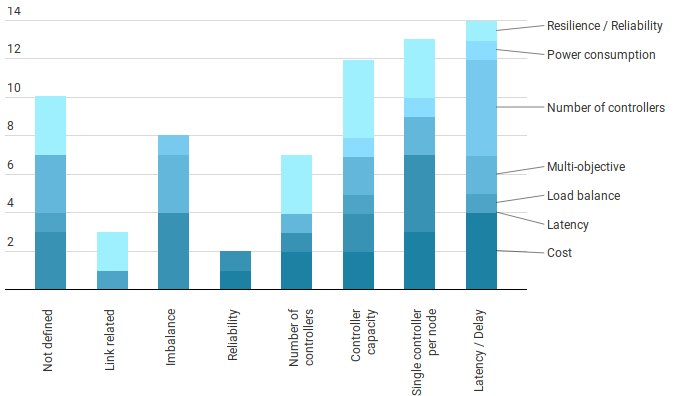
\includegraphics[width=0.45\textwidth]{Pictures/fig2.png}
    \caption{Constraits of the different \delia{purposes} \modia{optimization objectives}}
    \label{fig:constraint_purposes}
\end{figure}
%image  https://datawrapper.dwcdn.net/Ut9un/1/

\end{document}